\documentclass{brandeis-thesis3.2}
\usepackage[utf8]{inputenc}

\usepackage{hyperref}
\usepackage[round]{natbib}
\usepackage[nolist,nohyperlinks]{acronym}
\renewcommand{\bibsection}{\chapter*{References}\addcontentsline{toc}{chapter}{References}
}
\setcounter{secnumdepth}{5}
\usepackage{romannum}
\usepackage{amssymb}
\usepackage{amsmath}
\usepackage{wasysym}
\usepackage{tabularx} % extra features for tabular environment
\usepackage{graphicx} % takes care of graphic including machinery
\usepackage{subcaption} % from Jason: subfigures
\usepackage{float} % from Jason: better figure control



% short cuts
\def \msun {M_{\odot}}
\newcommand{\iso}[2]{$^{#1}${#2}}
\newcommand{\del}[3]{\delta^{#1}\text{#3}_{#2}}

\bibliographystyle{aasjournal}
\title{The Impact of Nuclear Uncertainties on the Galactic Chemical Evolution of Silicon Isotopes}
\author{Hung Kwan Fok}

\graduationmonth{May}
\graduationyear{2023}

\program{
  Undergraduate Program in Physics \\
  Department of Physics
}

\degreetype{Science}

% define acronym
\acrodef{gce}[GCE]{galactic chemical evolution}


\begin{document}

\maketitlepage
\makecopyright

\thispagestyle{empty}
\begin{center}
\vspace*{1cm}
    
    This Senior Honors thesis, directed and approved by Hung Kwan Fok' Committee, has been accepted and\\
    approved by
        
    \vspace{0.75cm}
    the Department of Physics at Brandeis University
        
    \vspace{0.75cm}
    in partial fulfillment of the requirements for the degree of: Bachelor of Science in Physics
    
    \vspace{2cm}
    \noindent\rule{14cm}{0.4pt}\\
    Dr. Aparna Baskaran, Undergraduate Advising Head
    
    \vspace{2cm}
    
    Committee Members:\\
    Dr. Reto Trappitsch, Dr. James Cho
    
    \vspace{2cm}
    
    


    \noindent\begin{tabular}{ll}
    \makebox[3in]{\hrulefill} & \makebox[3in]{\hrulefill}\\
    Printed Name & Signature\\[8ex]% adds space between the 2 sets of signatures
    \makebox[3in]{\hrulefill} & \makebox[3in]{\hrulefill}\\
    Printed Name & Signature\\
    \end{tabular}
\end{center}

\chapter*{Acknowledgments}
\addcontentsline{toc}{chapter}{Acknowledgments}
\begin{doublespacing}
I would like to express my deep and sincere gratitude to my committee members Professor Reto Trappitsch and Professor James Cho for their help and guidance on my work and their support in the past one year. I would also like to thank Professor Reto Trappitsch for offering me this great research opportunity. I would also like to extend my gratitude Dr. Marco Pignatari for his enormous help on my research. I would also like to thank Dr. Benoit Cote for his help on the GCE calculation and the OMEGA+ code. In addition, I would like to thank the NuGrid collaboration for developing the nucleosynthesis code PPN and GCE code OMEGA+ used in my work. 

\end{doublespacing}

% Page must be manually cleared before and after abstract since it's not a section/chapter as-is
\clearpage

\begin{thesis-abstract}
\addcontentsline{toc}{chapter}{Abstract}
 The Si isotopic composition of the mainstream SiC grains are believed to carry the galactic chemical evolution (GCE) signature. Measurements of Si isotope ratios in mainstream SiC grains suggest that there is a linear correlation between \iso{29}{Si}/\iso{28}{Si} and \iso{30}{Si}/\iso{28}{Si}. However, current GCE models have so far failed to explain the slope of that correlation line. This study aims to investigate how nuclear uncertainties affect the GCE of Si isotopes, specifically their ratios. A sequence of tasks are carried out. First, the stars responsible for the production of Si isotopes are identified. Second, the main Si production regions in those stars are identified, along with the relevant Si production and destruction reactions in those regions. Third, the impact of nuclear uncertainties on the nucleosynthesis of Si isotopes in the relevant regions and on the resulting modified stellar yields is calculated by varying the relevant reaction rates. Finally, the GCE of Si isotopes are calculated using the modified stellar yields. Through these four tasks, I have found that the nuclear uncertainties lead to a $\sim$5\% variation on the slope of the Si-correlation line. However, the slope I determined is more than a factor of three lower when compared with presolar grain measurement \citep{Zinner2007}; these authors calculated a slope of $1.37\pm 0.01$. This is likely due to the overestimation of \iso{30}{Si} production in convective oxygen-carbon shell mergers occurred in the 1D stellar evolution models. For the first time, my study quantified the effects of nuclear uncertainties on the GCE of isotopes.

\end{thesis-abstract}

% Page must be manually cleared before and after abstract since it's not a section/chapter as-is
\clearpage

\tableofcontents
\clearpage

% \listoftables
% \addcontentsline{toc}{chapter}{List of Tables}
% \clearpage

% \listoffigures
% \addcontentsline{toc}{chapter}{List of Figures}
% \clearpage

\startbody


\chapter{Introduction}

The major group of presolar SiC grains, the so-called mainstream grains, are believed to have condensed in the outflows of low-mass stars (up to a few solar masses) when they went through the asymptotic giant branch (AGB) phase at the end of their lives. However, the Si isotopic ratios measured in these grains cannot be explained in terms of the nucleosynthesis in AGB stars. Thus, the grains are believed to carry the signature of galactic chemical evolution (GCE). In particular, the Si isotopic composition of mainstream SiC grains represents overall nucleosynthesis in massive stars over roughly 9 billion years of GCE. Therefore, the Si isotopic composition measurements of the mainstream grains are a useful test on GCE models. Measurements of Si isotope ratios in mainstream SiC grains suggest that there is a linear correlation between \iso{29}{Si}/\iso{28}{Si} and \iso{30}{Si}/\iso{28}{Si}. However, current GCE models have so far failed to explain the slope of that correlation line. Past studies show that nuclear reaction rate uncertainties might be able to explain the discrepancy between the GCE model predictions and the mainstream grains measurements (\cite{Timmes_1996}; \cite{Hoppe_2009}). However, the effects of nuclear uncertainties on the GCE of Si isotopes have never been quantified. Therefore, this will be the focus of my work.

In my work, I aim to quantify the effect of nuclear uncertainties on the GCE of Si isotopes in a more physical way using a Monte Carlo method. In this chapter, I first give introduction to GCE and current GCE models (Section \ref{gce intro}). Then, I present different types of presolar grains, in particular, the SiC grains (Section \ref{grain intro}). Finally, I relate the Si isotopes measurements in the mainstream SiC grains with GCE to put my work in a broader context and layout the steps in my work (Section \ref{m gce intro})).

\section{Galactic Chemical Evolution} \label{gce intro}

\Ac{gce} refers to the evolution of elements and isotopes in the galaxy. In this section, I discuss the basic ingredients of \ac{gce} models and the different types of models used for GCE.

\subsection{Basic Ingredients}

There are four necessary ingredients for a typical GCE model: initial conditions, the stellar birthrate function, the nucleosynthesis yields recycled back into the galaxy, and gas inflow and outflow from the galaxy. The chemical abundance of an element $X_i$ over time is used, and is given by:

\begin{equation} \label{eq:massfrac}
X_i = \frac{M_i}{M},
\end{equation}
where $M_i$ is the mass of the element in the interstellar medium (ISM), and $M$ is the total mass of the gas.

The initial conditions of a GCE model refer to the initial composition of the galaxy. One typical initial composition is the primordial abundance, i.e. the the elements formed in the Big Bang which mainly consist of elements lighter than lithium. The initial composition of a GCE model can also be a metal-enriched chemical composition, known as prompt initial enrichment (PIE), which is enriched by an initial generation of the first stars that were only composed of primordial material. In astronomy, metal refers to the elements that are heavier than hydrogen and helium. The metallicity $Z$ is then defined by the mass fraction of the elements heavier than hydrogen and helium.

The stellar birthrate function describing the number of stars formed in the time interval $(t, t+\Delta t)$ and in the mass interval $(m, m+\Delta m)$ in a galaxy can be written as
\begin{equation}
B(m, t) \Delta m \Delta t= \psi (t) \phi(m) \Delta m \Delta t,
\end{equation}
where $\psi (t)$ is the star formation rate (SFR) and $\phi (m)$ is the initial mass function (IMF). The SFR represents the rate at which stars form from interstellar gas. A common parameterization of the SFR is given by the Schmidt-Kennicutt law (\citealt{schmidt}),

\begin{equation}
\psi (t) = \nu \sigma_{\rm gas}^{k},
\end{equation}
where $\nu$ is the star formation efficiency, $\sigma_{\rm gas}$ is the gas surface mass density, and $k$ is an exponential factor. The value of $k$ is $1.4\pm 0.15$, as determined by \cite{kennicutt}. The IMF describes the number distribution of stars with masses between $0.1\, \msun$ and $100\, \msun$. The first IMF was published by \cite{salpeter55}. More modern IMFs used in GCE models are published by \cite{kroupa01} and \cite{chabrier03}. A comparison between the three IMFs is shown in Figure \ref{fig:imf}.

\begin{figure}[H]
\centering
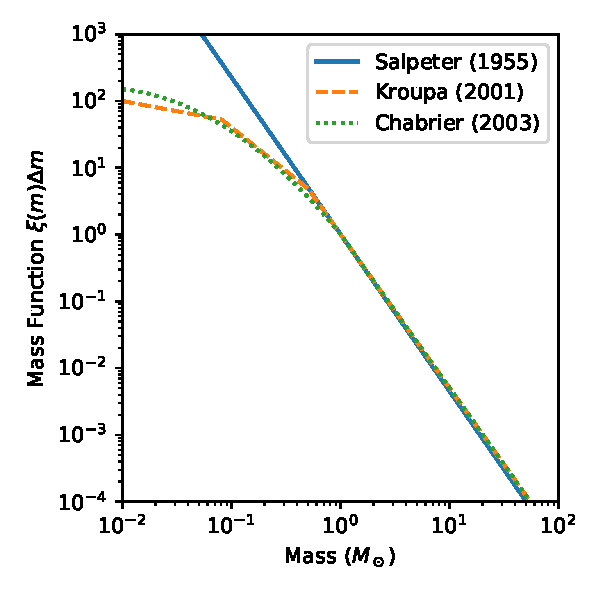
\includegraphics[width = 0.6\textwidth]{figs/imf.pdf}
\caption{Initial mass functions by \cite{salpeter55}, \cite{kroupa01}, and \cite{chabrier03}.}
\label{fig:imf}
\end{figure}


Stellar nucleosynthesis yields are another important input for GCE models. The chemical enrichment in galaxies is due to the chemical elements produced in stars and recycled back to the ISM when they die. The nucleosynthesis yield of a star depends on its mass. For stars with $M<0.8\,\msun$, their lifetime exceeds the Hubble time. The Hubble time is the time required for the universe to expand to its present size, assuming the Hubble constant has remained unchanged since the Big Bang. Therefore, they can only lock up gas and have limited contribution to GCE. Low- and intermediate-mass stars with $0.8\,\msun < M \lesssim 8 \, \msun$ form some $\alpha$-elements (i.e. elements that are mainly synthesized by $\alpha$-capture processes) and are the main site for the slow neutron capture process ($s$-process), which produces heavy elements (e.g. Ba, Sr, Y) by neutron addition to the \iso{56}{Fe} seed. These stars die as a CO white dwarf (WD) and leave behind a planetary nebula. The material in the CO WD is locked up, while the material in the planetary nebula is recycled back into the ISM. In binary systems, intermediate stars can die as Type Ia SNe (SNe-Ia). SNe-Ia significantly contribute to the iron-peak elements. However, since they require two fully evolved stars, they can only contribute on a large timescale. Massive stars with $8\,\msun<M<10\,\msun$ likely explode as electron-capture supernovae (ECSNe). However, the detailed mechanism behind ECSNe is still largely unknown. Massive stars with $M>10\,\msun$ are expected to explode as core-collapse supernovae (CCSNe). Massive stars with $8\,\msun<M\lesssim 25\,\msun$ mainly produce $\alpha$-elements, iron-peak elements, and part of the \textit{s}-process elements. It is argued that CCSNe can host rapid neutron processes (\textit{r}-processes) and can contribute to the production of proton-rich nuclei (\textit{p}-nuclei). 

Other events can also contribute to GCE. For example, neutron star mergers (NSM) are thought to be one of the most promising channel for r-process element production (\citealt{Korobkin_2012}; \citealt{Eichler_2015}). However, these production events likely have minor effect on the overall GCE. 

When building a realistic model of a galaxy, it is important to consider the inflow and outflow of gas. GCE models that do not take into account these processes are known as closed-box models. The main effect of gas inflow and outflow in GCE models is to change the metallicity of the galaxy. Gas inflows are generally considered to be either gas accretions or radial gas flows. Typically, gas is assumed to flow in from the metal-poor halo, which has a primordial composition, as the material in the halo has not been processed through the GCE. Primordial composition is the elemental composition from the big bang nucleosynthesis. Gas outflows also change the metallicity of the galaxy by reducing the amount of gas available for star formation. Galactic gas outflows are primarily caused by SNe, which accelerate the gas and transport it away from the galactic disk.

\subsection{Galactic Chemical Evolution Models}

The one-zone model is one of the simplest GCE models. In this model, the materials released from stars are immediately recycled back into the galaxy. The evolution of an element $X_i$ as a function of time can be written as:

\begin{equation}
\frac{d(X_if_g)}{dt} = \sum_{\rm event} E_{\rm event} - X_i\psi + X_{i, in}R_{in} - X_iR_{out}.
\end{equation}
Here, $f_g$ is the fraction of mass that is in gas form. $\sum_{\rm event} E_{\rm event}$ represents the sum over the contribution from all production events. $X_{i, in}$ is the mass fraction of element $i$ in the inflow gas, and $R_{in}$ is the inflow rate, while $R_{out}$ is the outflow rate. Although the one-zone model is a good first-order approximation, it cannot track the heterogeneous evolution of the galaxy due to the instantaneous mixing assumption. However, it is a simple and self-consistent way to track the evolution of all the elements.

In contrast to one-zone models, chemodynamical models do not assume that stellar feedback is instantaneously available throughout the entire galaxy. Instead, each nucleosynthesis event is modeled using star particles, and feedback from these particles is mixed in the galaxy using a hydrodynamical prescription (e.g., \citealt{Kobayashi_2015}). Each star particle is an association of many stars, and its chemical composition represents the local average within the given star particle. 

Note that because one-zone models are computationally-fast, they can be combined with a Markov Chain Monte Carlo (MCMC) code to study uncertainties and the impact of modeling assumptions in the GCE model. \cite{cote17} presents a simple GCE code, One-zone Model for the Evolution of GAlaxies (OMEGA), which, when combined with an MCMC calculation, reproduced the observed abundance evolution of O, Mg, Si, Ca, Ti, Cr, Mn, Ni, and Co in Sculptor, a dwarf spheroidal galaxy. This dwarf galaxy is chosen since it has been simulated many times in the past (\citealt{Vincenzo_2014}, \citealt{Homma_2015}, \citealt{Kobayashi_2015}) and is thus a good test case for the OMEGA model. \cite{cote17} find the best set of parameters, along with their confidence levels. They conclude that chemical evolution results in this case are primarily affected by the stellar nucleosynthesis yields used, rather than the complexity of the dwarf galaxy model itself. Therefore, simple one-zone models can sufficiently constrain GCE and validate stellar nucleosynthesis models.

\section{Presolar Grains} \label{grain intro}
\subsection{The origin of Presolar Grains}
Presolar grains are solid materials that formed in the outflows of dying stars and were subsequently mixed into the interstellar medium. During the formation of the solar system, presolar grains were incorporated into meteorite parent bodies and can today be found in and extracted from primitive meteorites. Figure \ref{fig:presolar_origin} shows a schematic of the history of presolar grains. Presolar grains contain the nucleosynthesis signature of their parent star, and we can analyze their isotopic composition with high-precision. Therefore, they are useful in constraining GCE and stellar nucleosynthesis models, at least for simple systems such as Sculptor.

\begin{figure}[H]
\centering
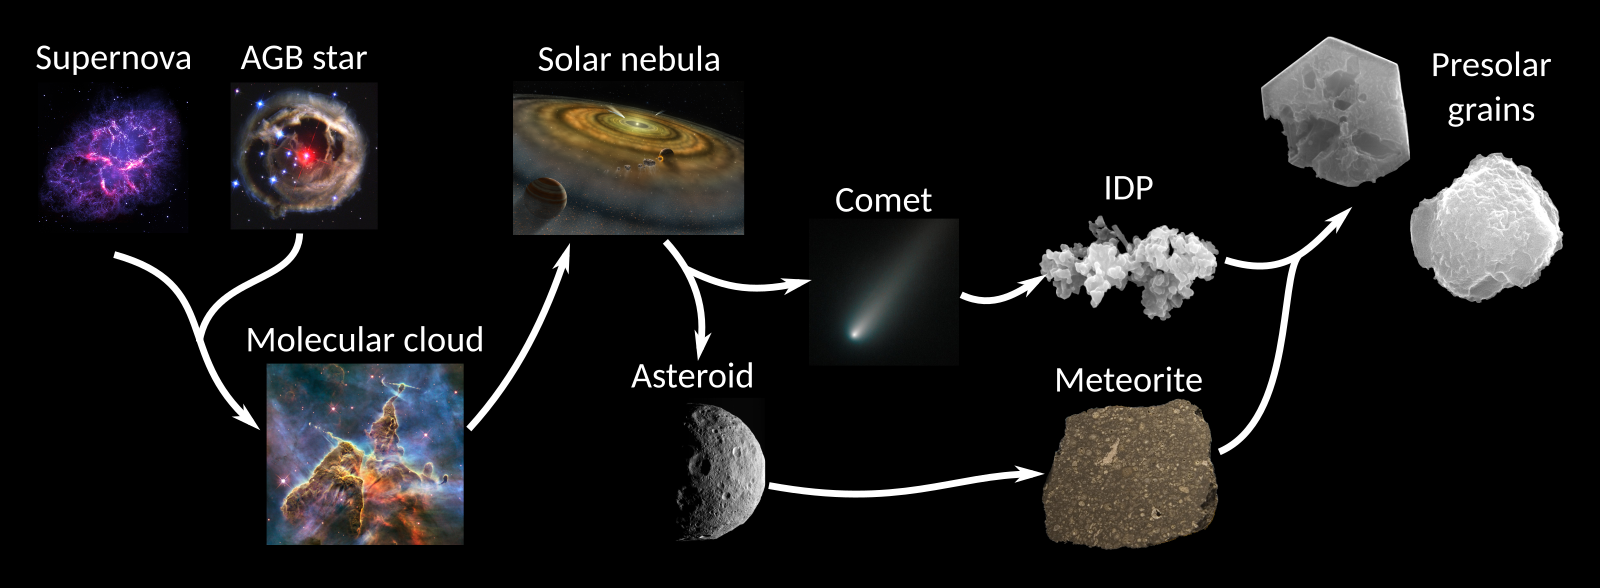
\includegraphics[width = 0.9\textwidth]{figs/presolar_grains_origin_1600.png}
\caption{Schematic of the origin of presolar grains.}
\label{fig:presolar_origin}
\end{figure}

\subsection{Types of Presolar Grains}
One of the best-studied presolar grain phases is silicon carbide (SiC) (Figure \ref{fig:sic_pic}). These SiC grains occur in sizes of up to several micrometers, can be separated from meteorites, and studied individually in the laboratory. Other types of presolar grains include nanodiamonds and graphite grains. Nanodiamonds are the most abundant type of presolar grains. However, these particles are only tens of nanometers in diameter and can therefore not be studied individually in the laboratory. Graphite grains can also be separated from meteorites. They also occur in large sizes. However, they often show contamination with solar system material.

\subsection{Silicon Carbide Grains}
Measurements of SiC grains can be particularly useful in constraining stellar nucleosynthesis and GCE models. These grains are generally analyzed by mass spectrometry for their isotopic composition. The isotopic measurement is usually expressed as ratios with respect to the most abundant isotope in $\delta$-notation,
\begin{equation}
\delta^i X_j = \delta\left(\frac{^iX}{^jX}\right) = \left[ \frac{\left( \frac{^iX}{^jX}\right)_{sample}}{\left(\frac{^iX}{^jX}\right)_{\odot}} - 1\right] \times 1000\ (\permil)
\end{equation}

\begin{figure}[H]
\centering
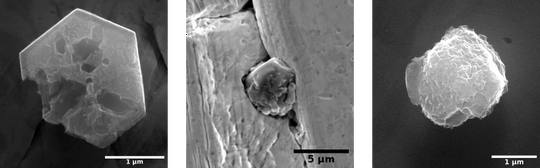
\includegraphics[width= 0.9\textwidth]{figs/stardust.png}
\caption{Secondary electron images of three different SiC grains that were extracted from the Murchison meteorite.}
\label{fig:sic_pic}
\end{figure}

Based on their C, N, and Si isotopic composition, SiC grains can be divided into different groups (Figure \ref{fig:sic}). Most of the SiC grains belong to the so-called mainstream (M) group. The mainstream grains are believed to come from $1.5-3\,\msun$ AGB stars with roughly solar metallicity. Another important type of presolar SiC grains are the so-called X grains, which are characterized by an enhancement in \iso{28}{Si}, \iso{12}{C}, and \iso{15}{N} with respect to the solar composition, as shown in Figure \ref{fig:sic}. X grains are believed to have formed in the ejecta of core-collapse supernovae. Other types of SiC grains of likely SNe origin are grains of type AB, C, X, and nova. 

\begin{figure}[H]
     \centering
     \begin{subfigure}[b]{0.48\textwidth}
         \centering
         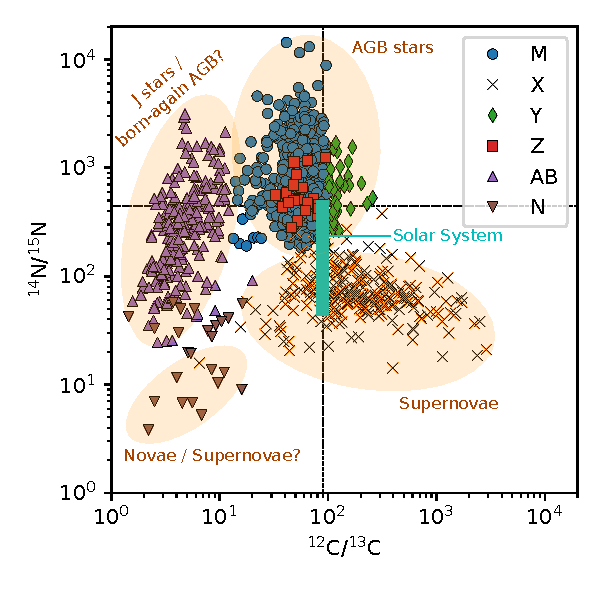
\includegraphics[width=\textwidth]{figs/sic_n_c_all.pdf}
        %  \caption{}
     \end{subfigure}
     \begin{subfigure}[b]{0.48\textwidth}
         \centering
         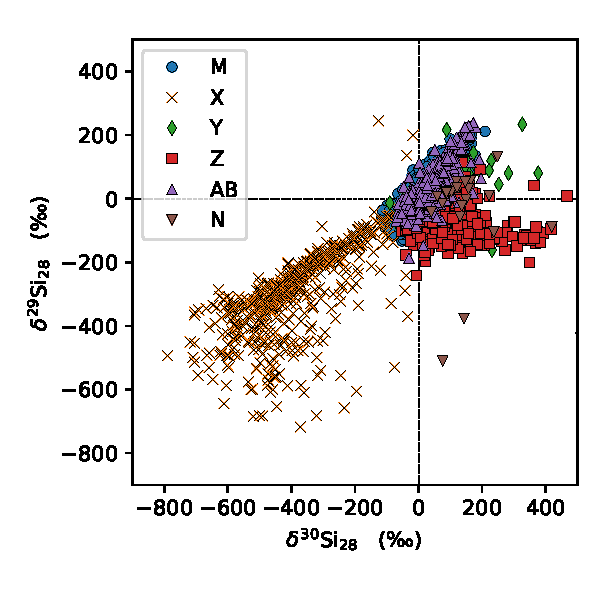
\includegraphics[width=\textwidth]{figs/sic_si_3iso_all.pdf}
        %  \caption{}
     \end{subfigure}
     \caption{(Left) Nitrogen and carbon isotopic composition of analyzed SiC grains. Presolar grain groups are identified in the legend. The green line represents all measurements of the solar system material. (Right) Silicon isotopic composition of SiC grains. The measurements are shown in $\delta$-notation \citep[data from][]{stephan_20}.}
     \label{fig:sic}
\end{figure}

\section{Silicon Isotopes in Mainstream Grains and GCE} \label{m gce intro}
The silicon isotopic composition of the mainstream grains is characterized by enrichment in heavy silicon isotopes of up to $\sim200\permil$ relative to the solar system composition. Moreover, in the so-called silicon three-isotope plot, the mainstream grain data show a correlation between their \iso{29}{Si}/\iso{28}{Si} and \iso{30}{Si}/\iso{28}{Si} ratios. In particular, they plot along the so-called Si mainstream line $\del{29}{28}{Si} = 1.37 \times \del{30}{28}{Si} -20\permil$ (\citealt{Zinner2007}). Although the mainstream grains come from AGB stars, their silicon isotopic ratios cannot be explained by nucleosynthesis in their parent stars (\citealt{Lugaro1999}). Instead, the Si mainstream line represents the GCE of silicon isotopes. However, current GCE models fail to explain their silicon isotopic abundances. There are three main problems:
\begin{enumerate}
    \item The scatter in the Si isotopic compositions of the parent stars shown by the mainstream grains measurements cannot be explained by the classical GCE model;
    \item Most of the mainstream grains have higher than solar \iso{29}{Si}/\iso{28}{Si} and \iso{30}{Si}/\iso{28}{Si} ratios. In the classical GCE picture, the \iso{29}{Si}/\iso{28}{Si} and \iso{30}{Si}/\iso{28}{Si} ratios increase with metallicity $Z$, which is a proxy for time.
    \item The slope of the Si mainstream line is larger than the prediction by the GCE models. The slopes predicted by most GCE models are $\sim$1.
\end{enumerate}

% \begin{figure}[H]
%     \centering
%     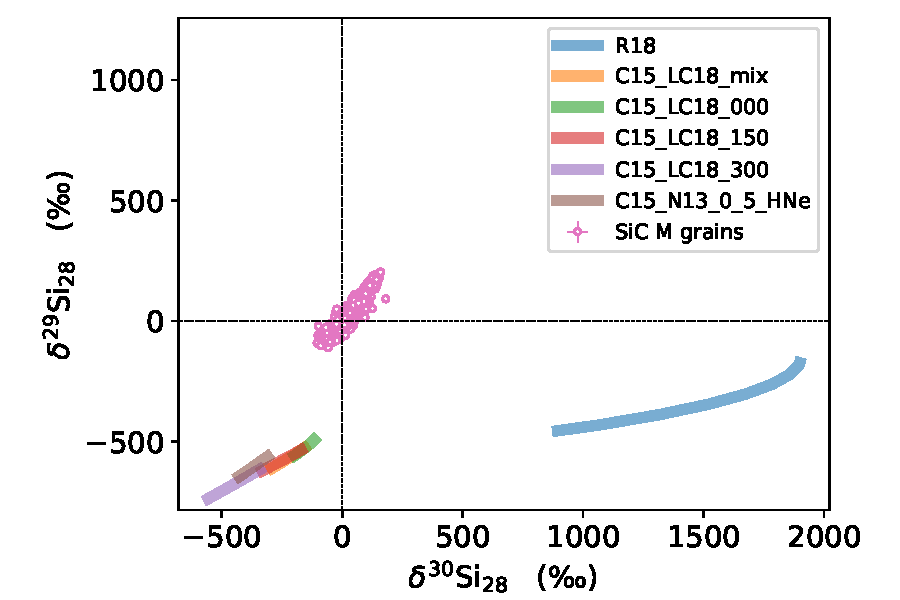
\includegraphics[width = 0.75\textwidth]{figs/gce_Si_isotope.pdf}
%     \caption{Comparison between the GCE model and the mainstream grain data. GCE is simulated using OMEGA+ (\citealt{Cote_2018}) with different stellar yield sets available in the JINAPyCEE\protect\footnotemark  package.}
%     \label{fig:gce_si}
% \end{figure}

Different solutions are proposed for the first two problems. \cite{Lugaro1999} explain the scatter using local heterogeneities in the regions from which the parent stars of the mainstream grains originally formed due to the stochastic nature of the admixture of the contributions from supernovae of varying mass and type. However, this model breaks down when other GCE-dominated isotopes (e.g., Ti isotopes) in the mainstream grains are investigated \citep{Nittler_2005}. \cite{Clayton1997} addresses the second problem by considering star migration. The mainstream grains might have originated from stars that were born in central, more metal-rich regions of the galaxy and moved to the molecular cloud from which the solar system is formed.\footnote[1]{https://github.com/becot85/JINAPyCEE}

In my study, I will focus on the third problem, namely the discrepancy between the slope of the Si mainstream line and the slope predicted by GCE models. There are indications that the nuclear uncertainties in stellar nucleosynthesis calculations might be able to explain the problem (\citealt{Timmes_1996}; \citealt{Hoppe_2009}). In particular, \cite{Timmes_1996} points out that the abundances of the Si isotopes in the ISM are largely determined from CCSNe ejecta. These authors also indicate that the key nuclear reaction rates affecting the abundance of neutron-rich Si isotopes in CCSNe might have systematic errors. Moreover, \cite{Hoppe_2009} shows that increasing the rate of \iso{26}{Mg}$(\alpha, n)$\iso{29}{Mg} by a factor of 3 will lead to an increase in the \iso{29}{Si}/\iso{28}{Si} by a factor of 1.8 with the \iso{30}{Si}/\iso{28}{Si} ratios largely unchanged. Such an increase is able to explain the Si isotopic abundance measured in an individual presolar grain, which is believed to originate from a CCSN (\citealt{Hoppe_2009}). However, the effects of nuclear uncertainties on the GCE of isotopes have never been quantified. This will be the focus of my work. In my work, I aim to quantify the effect of nuclear uncertainties on the GCE of Si isotopes in a more physical way using a Monte Carlo method. The steps in my work can be summarized as follows:
\begin{enumerate}
    \item Identify the stars that are responsible for the production of silicon isotopes in the galaxy.
    \item Identify the main Si-production regions in those stars and the relevant reactions for Si production and destruction.
    \item Calculate the nucleosynthesis in the relevant regions and the resulting stellar yield with varying reaction rates.
    \item Calculate the GCE of Si isotopes using the modified stellar yields.
\end{enumerate}

Through these steps, I aim to answer the question if nuclear uncertainties can explain the model-data discrepancy of the Si isotopic ratios observed in the presolar SiC mainstream grains. In chapter \ref{method}, I discuss the numerical models I used for nucleosynthesis and GCE calculations and the pipeline I developed connecting the models, as well as the Monte Carlo setup. In chapter \ref{pre-result}, I discuss the nucleosynthesis of Si isotopes in stars. I identify the stars responsible for Si production in the galaxy, as well as relevant stellar regions and nuclear reactions for Si-production. In chapter \ref{mc_result}, I show Monte Carlo result of nucleosynthesis and GCE. I compare the GCE result with the mainstream grain data. In chapter \ref{conclusion}, I summarize the main results and discuss the implications and future work.



\chapter{Method} \label{method}

In this chapter, I discuss the numerical models and methods I used in my study. In Section \ref{nucleosynthesis}, I discuss the numerical model I used for the stellar nucleosynthesis calculations. In Section \ref{yield}, I discuss the calculation I used to determine the integrated stellar nucleosynthesis yields from the nucleosynthesis calculations. In Section \ref{gce}, I discuss the numerical model I used for the GCE simulations. In Section \ref{pipeline}, I show the workflow of the pipeline connecting the stellar nucleosynthesis simulation to the GCE simulation. In Section \ref{mc}, I show the Monte Carlo setup I used to quantify the effects of the nuclear uncertainties on the GCE of Si isotopes.

\section{Nucleosynthesis Simulation} \label{nucleosynthesis}
I use a post-processing approach in the nucleosynthesis simulations in my work. In the post-processing approach, the stellar evolution is simulated using a reduced nuclear network that is large enough to account for the nuclear energy generation. The stellar evolution data for all zones at all time steps are then post-processed using a full nuclear network for nucleosynthesis calculation. This is done at one mass coordinate (with the single-zone code PPN) or for an entire star (with the multizone code MPPNP). In my work, the single-zone code PPN is used. In the case of the single-zone code PPN, changes in temperature $T$ and density $\rho$ with time in the chosen zone -- the so-called trajectory, which can be extracted from the stellar model -- have to be provided. The initial condition for the network calculation is the initial mass fractions of isotopes. The isotopic mass fractions are then evolved using the full nuclear network and the provided trajectory. A sample result from a PPN run is shown in Figure \ref{fig:ppn_sample}. To get a consistent result, the post-processing network needs to use the same nuclear physics for energy-generating reactions as is used in the stellar evolution calculation.

\begin{figure}[h]
\centering
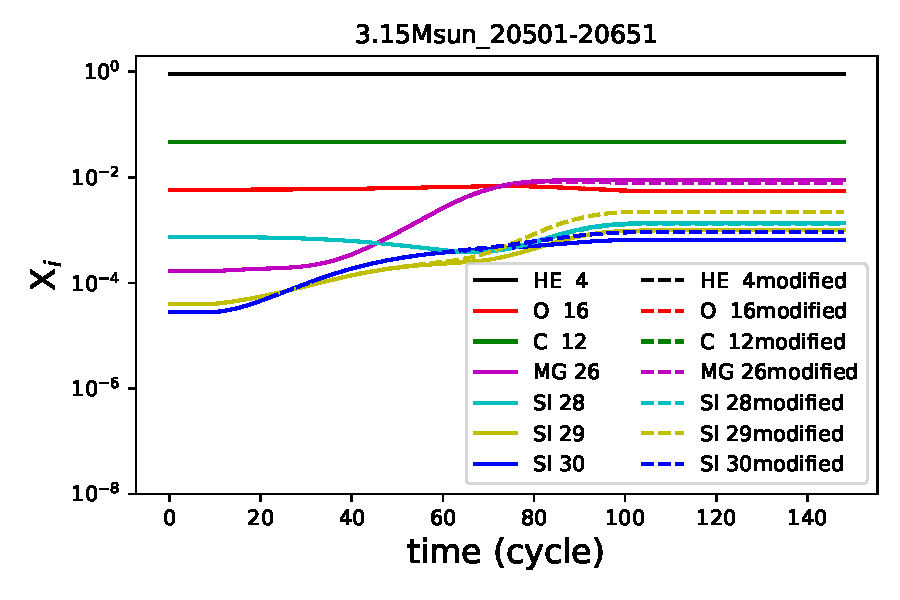
\includegraphics[width=0.8\textwidth]{figs/ppn_sample.pdf}
\caption{A sample PPN result. The solid lines represent the evolution of the isotopic abundances using the default nuclear reaction network. The dashed lines represent the evolution of the abundances with the rate of \iso{26}{Mg}$(\alpha,n)$\iso{29}{Si} increase by a factor of 3. The trajectory used is an explosive trajectory (i.e., the trajectory from a CCSN model). The trajectory is taken from the stellar model with initial mass $M=15\msun$ and initial metallicity $Z=0.02$ at the mass coordinate $m=3.15\,\msun$ for model steps $20501-20651$. The initial abundance is the pre-supernova abundance. PPN then follows the nucleosynthesis throughout the explosion.}
\label{fig:ppn_sample}
\end{figure}

I obtain the stellar structure evolution data (trajectory) from the NuGrid models. NuGrid models refer to the stellar evolution and nucleosynthesis models in \cite{Pignatari_2016} and \cite{Ritter_2018}. These models use the MESA stellar evolution code (\citealt{Paxton_2011}) for the stellar evolution calculations. In my work, I use the delayed-convection explosions recipe from \cite{Fryer_2012} for the CCSNe explosions, and the semi-analytic approach with the shock launched from the protoneutron stars based on a mass cut derived from \cite{Fryer_2012} is used in the NuGrid models for the CCSN explosions.



\section{Integration of Stellar Nucleosynthesis Yields} \label{yield}
To incorporate the single-zone PPN results into the GCE simulation, it is necessary to compute the integrated stellar nucleosynthesis yields using these results.

In my model, the zones are identified by their mass coordinate, $m_i \in {m_0, m_1, ..., m_M}$. From the mass range of interest, $[m_a, m_b]$, $N$ trajectories with mass coordinates $m_{a+n\delta}$ are selected, where $n<N$ and $\delta=(b-a)|N$. Note that $a, b, n\in \mathbb{N}$ and $b>a$. For each of the selected trajectories, I use PPN to compute the Si-yield scale factor $\lambda_{a+n\delta}$ for a given nuclear reaction rate modification. Then, for $a+n\delta\leq i \leq a+(n+1)\delta$, I obtain the scale factor at $m_i$ using linear interpolation,
\begin{align}
\lambda_i = \lambda_{a+n\delta} + (m_i-m_{a+n\delta})\cdot \left[ \frac{\lambda_{a+(n+1)\delta}-\lambda_{a+n\delta}}{m_{a+(n+1)\delta}-m_{a+n\delta}}\right].
\end{align}
For $i<a$ or $i>b$, $\lambda_i=1$. The integrated stellar nucleosynthesis yield is then computed by numerical integration as follows:
\begin{align}
\sum_{i=k}^{M-1} \lambda_i X_i \Delta m_i,
\end{align}
where $m_k$ is the mass cut derived from \cite{Fryer_2012}, $X_i$ is the isotopic mass fraction in the stellar nucleosynthesis models in \cite{Ritter_2018} (NuGrid nucleosynthesis models), and $\Delta m_i = m_{i+1}-m_i$.

\section{Galactic Chemical Evolution Simulations} \label{gce}

In this study, I utilize the 2-zone semi-analytic GCE model OMEGA+ (\citealt{Cote_2018}). The OMEGA+ model consists of a star-forming region, representing the galaxy, surrounded by a hot gas reservoir filling the dark matter halo of the host galaxy, known as the circumgalactic medium (CGM). I adopt the open-box one-zone GCE model OMEGA (\citealt{cote17}) to simulate the stellar population within the galaxy. The OMEGA code calculates the chemical composition of the interstellar medium (ISM) as a function of time using a given input star formation history. The calculation takes into account the contribution of multiple stellar populations, as well as the effect of galactic inflows and outflows. OMEGA+ interacts with OMEGA at each time step to regulate the rate of inflow, outflow, and star formation. 

\begin{figure}[H]
    \centering
    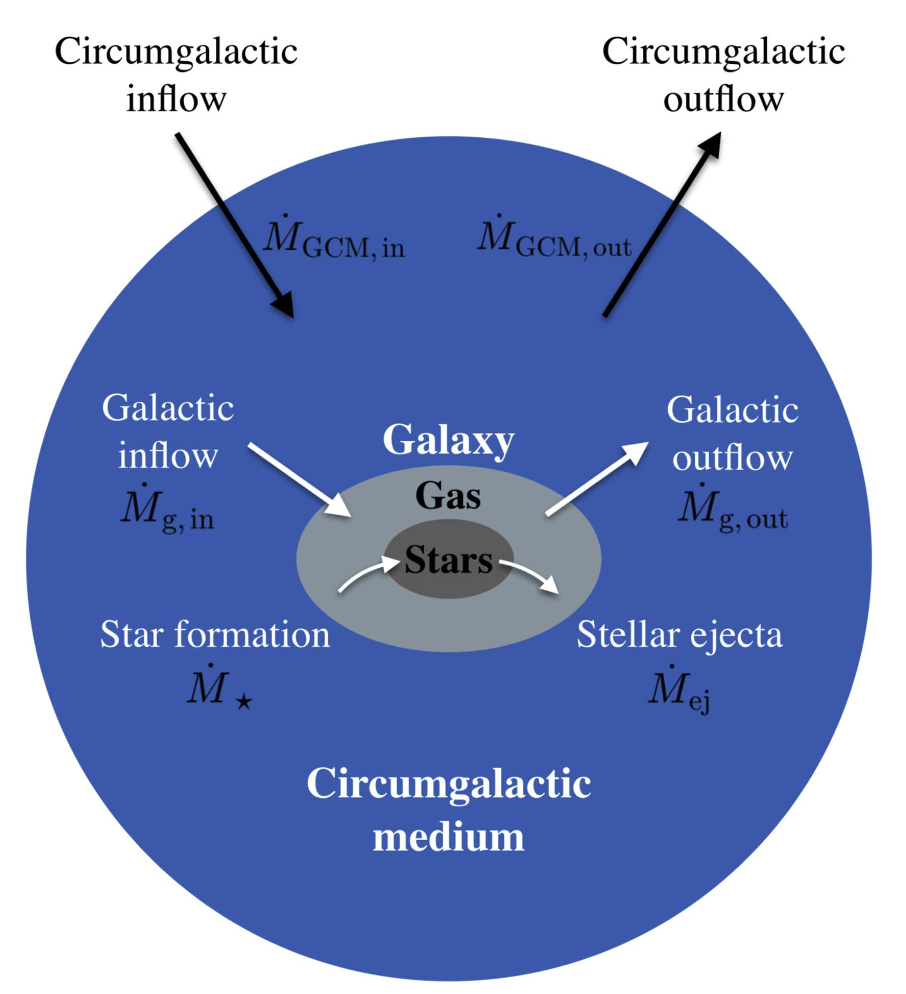
\includegraphics[width = 0.55\textwidth]{figs/omega.png}
    \caption{Structure overview of OMEGA+. The star-forming region is located at the center of the CGM. The arrows show the gas transfer processes in the model described in equation \ref{eq:galaxyflow} and \ref{eq:cgmflow}. Figure from \cite{Cote_2018}. }
    \label{fig:omega}
\end{figure}

The time evolution of the gas mass within the star-forming region, $M_{gas}$, is defined by the following equation:
\begin{align} \label{eq:galaxyflow}
\dot{M}_{gas} &= \dot{M}_{g, in} + \dot{M}_{ej} - \dot{M}_{*} - \dot{M}_{g, out},
\end{align}
where $\dot{M}_{g, in}$ represents the galactic inflow rate, $\dot{M}_{ej}$ is the mass-loss rate of all stars, $\dot{M}_{*}$ is the star formation rate, and $\dot{M}_{g, out}$ is the galactic outflow rate. The time evolution of the mass of the CGM, $M_{CGM}$, is defined by the following equation:
\begin{align} \label{eq:cgmflow}
\dot{M}_{CGM} &= \dot{M}_{CGM, in} + \dot{M}_{g, out} - \dot{M}_{g, in} - \dot{M}_{CGM, out},
\end{align}
where $\dot{M}_{CGM, in}$ represents the circumgalactic inflow rate, and $\dot{M}_{CGM, out}$ is the circumgalactic outflow rate. The galactic inflow rate is defined by
\begin{align}
\dot{M}_{g, in} = \frac{M_{CGM}}{\tau_{inflow}},
\end{align}
where $\tau_{inflow}$ is the inflow timescale. The circumgalactic inflow rate is defined by
\begin{align}
\dot{M}_{CGM, in} = \dot{M}_{DM} \left( \frac{\Omega_{M, 0}}{\Omega_{b, 0}} - 1\right)^{-1},
\end{align}
where $\dot{M}_{DM}$ is the growth rate of the dark matter mass and $\Omega_{b, 0}/\Omega_{M, 0}$ the universal baryonic fraction. The star formation rate is defined by
\begin{align}
\dot{M}_{*} = f_{*}M_{gas},
\end{align}
where $f_$ is the star formation efficiency. The galactic outflow rate is defined using the mass-loading factor $\eta_{gal}$, 
\begin{align}
    \eta_{gal} = \frac{\dot{M}_{g, out}}{\dot{M}_{*}}.
\end{align}
Similarly, the circumgalactic outflow rate can be defined using the mass-loading factor $\eta_{CGM}$, 
\begin{align}
    \eta_{CGM} = \frac{\dot{M}_{CGM, out}}{\dot{M}_{*}},
\end{align}
and is assumed to be proportional to the galactic outflow rate through the parameter $f_{\eta}$, 
\begin{align}
    \dot{M}_{CGM, out} = f_\eta \eta_{gal} \dot{M}_{*}.
\end{align}
The mass-loss rate of all stars $\dot{M}_{ej}$ is given by the stellar nucleosynthesis yields. 

\section{Pipeline} \label{pipeline}
I develop a pipeline that connects the stellar nucleosynthesis simulation to the GCE simulation. The pipeline is composed of three main parts: stellar nucleosynthesis simulation (Section~\ref{nucleosynthesis}), yield calculations for stellar nucleosynthesis, and GCE simulations (Section~\ref{gce}). The general workflow is depicted in  the flow diagram in Figure \ref{fig:workflow}.

\begin{figure}[H]
\centering
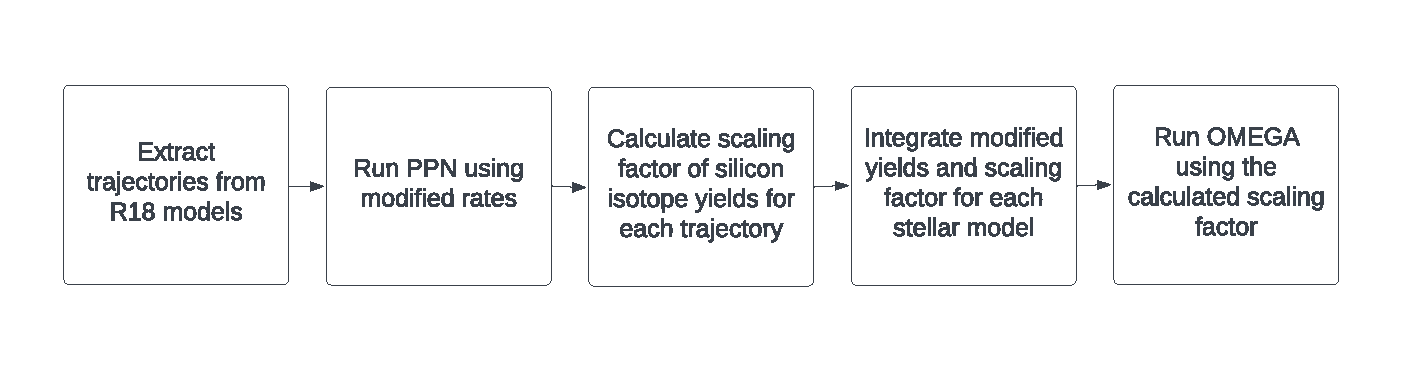
\includegraphics[width=\textwidth]{figs/Flowchart.pdf}
\caption{General workflow of the pipeline. Here, R18 models refer to the NuGrid models in \cite{Ritter_2018}.}
\label{fig:workflow}
\end{figure}

\section{Monte Carlo Method} \label{mc}
In this work, I combine the pipeline (\ref{pipeline}) with a Monte Carlo (MC) approach to vary nuclear reaction rates according to their uncertainties and model the effect of these rates on the GCE of silicon isotopes. MC is a numerical method that uses repeated random sampling to estimate the solution of a problem where uncertainties or randomness are present. It is widely used in many fields of science and engineering. However, many hydrodynamical simulations in astrophysics are computationally demanding. With the post-processing technique for single trajectories (PPN), I am able to limit the computation time of the nucleosynthesis simulations. Thus, performing a statistically sufficient number of MC calculations becomes feasible. 

I employ an MC method by drawing a set of random numbers to vary the relevant nuclear reaction rates simultaneously within predefined limits. This allows me to map the nuclear uncertainties onto the uncertainties in the final abundance of stellar nucleosynthesis via the reaction network and, finally, onto GCE simulations of silicon isotopes. 

\subsection{Rate Variation Factors}
For the uncertainties of stellar reaction rates, it is unavoidable to combine theoretical and experimental uncertainties. This is partly due to the fact that cross-sections of many reactions have not been measured. Therefore, the experimental uncertainties are used for some of the reactions while the theoretical uncertainties are used for others. In my setup, I vary rates by a certain factor smaller or larger than unity with respect to the default rates used in the NuGrid models. To combine the experimental and theoretical uncertainties, the rates are varied within predefined limits following a uniform distribution (\citealt{Rauscher_2016}). The limit for the experimental rates is given by $\pm 2\sigma$ where $\sigma$ is the experimental uncertainty. I use the uncertainty given in \cite{Rauscher_2016} for the theoretical rates. Table \ref{tab:rate} shows the variation factors for the theoretical rates.

\begin{table}[H]
    \centering
    \caption{Theoretical upper and lower limits assumed for different reaction types. For the upper and lower limit, the rate is multiplied by $U^{\rm hi}_{\rm th}$ and $U^{\rm lo}_{\rm th}$, respectively.}
\begin{tabular}{l c c}
        \hline
          Reaction &    $U^{\rm hi}_{\rm th}$ & $U^{\rm lo}_{\rm th}$\\
        \hline
        $(n,\gamma)$   & 2.0 & 2.0\\
        $(p,\gamma)$   & 2.0 & 3.0\\
        $(p,n)$         & 2.0 & 3.0\\
        $(\alpha,\gamma)$ & 2.0 & 10.0\\
        $(\alpha, n)$ & 2.0 & 10.0\\
        $(\alpha, p)$ & 2.0 & 10.0\\
        \hline
    \end{tabular}
    \label{tab:rate}
\end{table}



%%%%%%%%%%%%%%%%%%%
\chapter{Nucleosynthesis of Silicon Isotopes in Stars} \label{pre-result}

In this chapter, I identify the production sites of Si isotopes in the galaxy. In Section \ref{si_star}, I identify the stars that are responsible for the production of Si isotopes in the galaxy. In Section \ref{si_region}, I identify the main Si production regions in those stars.

\section{Silicon Production in the Galaxy} \label{si_star}
Since the production of silicon isotopes in stars depends on the initial mass and metallicity of the star, I first identify the stars that are responsible for silicon production in the Galaxy. To do so, I use the stellar nucleosynthesis yield set in \citealt{Ritter_2018} (NuGrid yield set) weighted by the initial mass function (IMF) from \cite{kroupa01}. It is necessary to weigh the stellar yields by the IMF because stars with different masses have different rates of occurrence in the galaxy, which changes their contribution to GCE. Here, I focus on stars with solar metallicity $Z=0.02$ and half-solar metallicity $Z=0.01$. 

Figure \ref{fig:imf_yield_0.02} shows the IMF-weighted stellar nucleosynthesis yield of \iso{28}{Si}, \iso{29}{Si}, and \iso{30}{Si} for stellar models with initial metallicity $Z=0.02$. For \iso{29}{Si} and \iso{30}{Si}, massive stars with initial mass $M_{ZAM}/\msun \geq 12$ are responsible for the majority of their production compared to other solar models. In particular, stars with initial mass $15 \leq M_{ZAM}/\msun \leq 20$ have the highest production in \iso{29}{Si} after being weighted by the initial mass function. Stars with $M_{ZAM}/\msun = 15$ have the highest production in \iso{30}{Si} after being weighted by the IMF. Figure \ref{fig:imf_yield_0.02} shows that stars with initial mass $15\leq M_{ZAM}/\msun \leq 20$ are the major source of \iso{29, \, 30}{Si} compared to other stars with the same initial metallicity $Z=0.02$.

Figure \ref{fig:imf_yield_0.01} shows the IMF-weighted stellar nucleosynthesis yield of silicon isotopes \iso{28}{Si}, \iso{29}{Si}, and \iso{30}{Si} for stellar models with initial metallicity $Z=0.01$. Similar to the case of $Z=0.02$, massive stars with $M_{ZAM}/\msun \geq 12$ are responsible for the majority of the production of these isotopes compared to other stellar models. In particular, stars with $M_{ZAM}/\msun = 15$ have the highest production in \iso{29}{Si} and \iso{30}{Si} after being weighted by the IMF. Figure \ref{fig:imf_yield_0.01} clearly shows that stars with initial mass $15\leq M_{ZAM}/\msun \leq 20$ are the most important source of \iso{29,\, 30}{Si} compared to other stars with the same metallicity $Z=0.01$. 

My result shows that massive stars are responsible for most of the silicon isotope production in the galaxy. In particular, since I am mainly interested in the production of \iso{29}{Si} and \iso{30}{Si}, I should focus on the nucleosynthesis in the stars with $15 \leq M_{ZAM}/\msun \leq 20$. This mass range corresponds to the NuGrid models with initial mass $M_{ZAM}/\msun = 15, 20$.
\begin{figure}[H]
    \begin{subfigure}[c]{0.6\textwidth}
        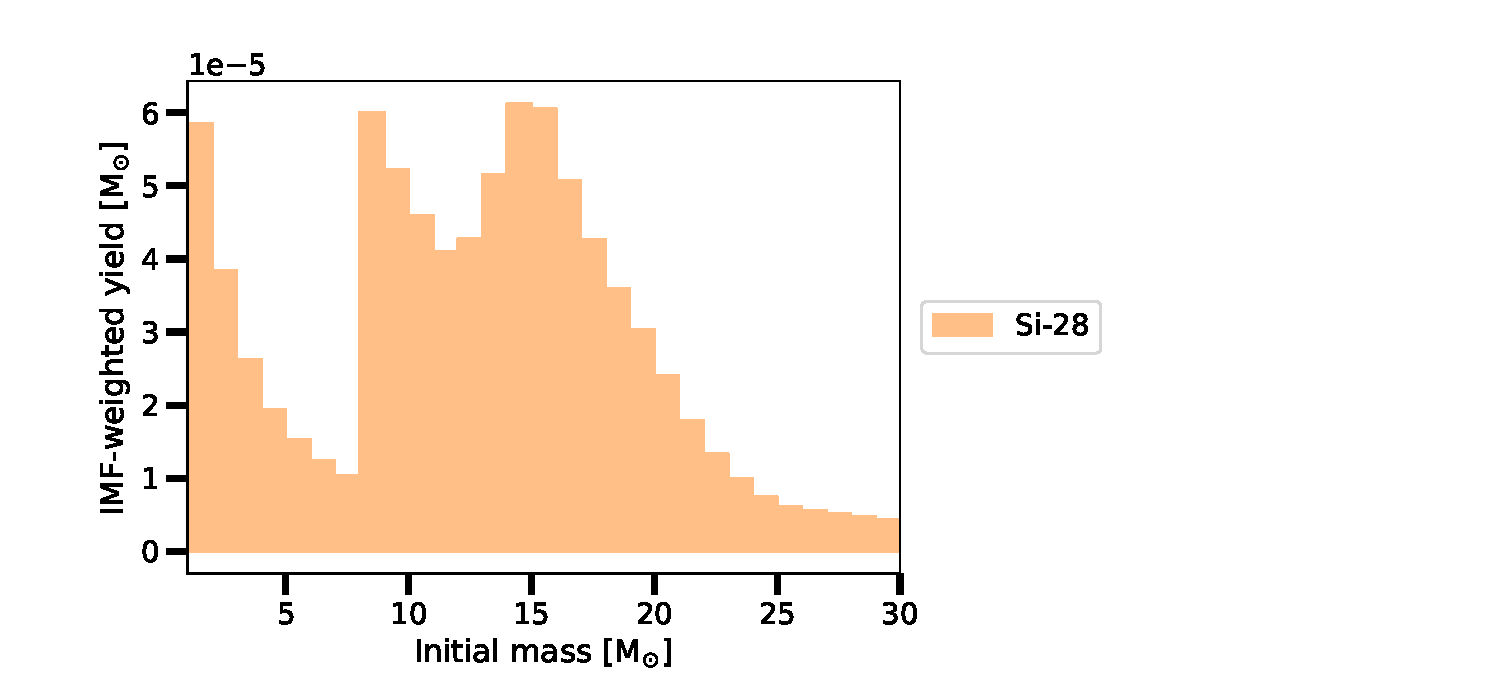
\includegraphics[width=\textwidth]{figs/Si-28_Z=0.02_yield.pdf}
        \caption{IMF-weighted stellar nucleosynthesis yield of \iso{28}{Si}.}
    \end{subfigure}
    \begin{subfigure}[c]{0.6\textwidth}
        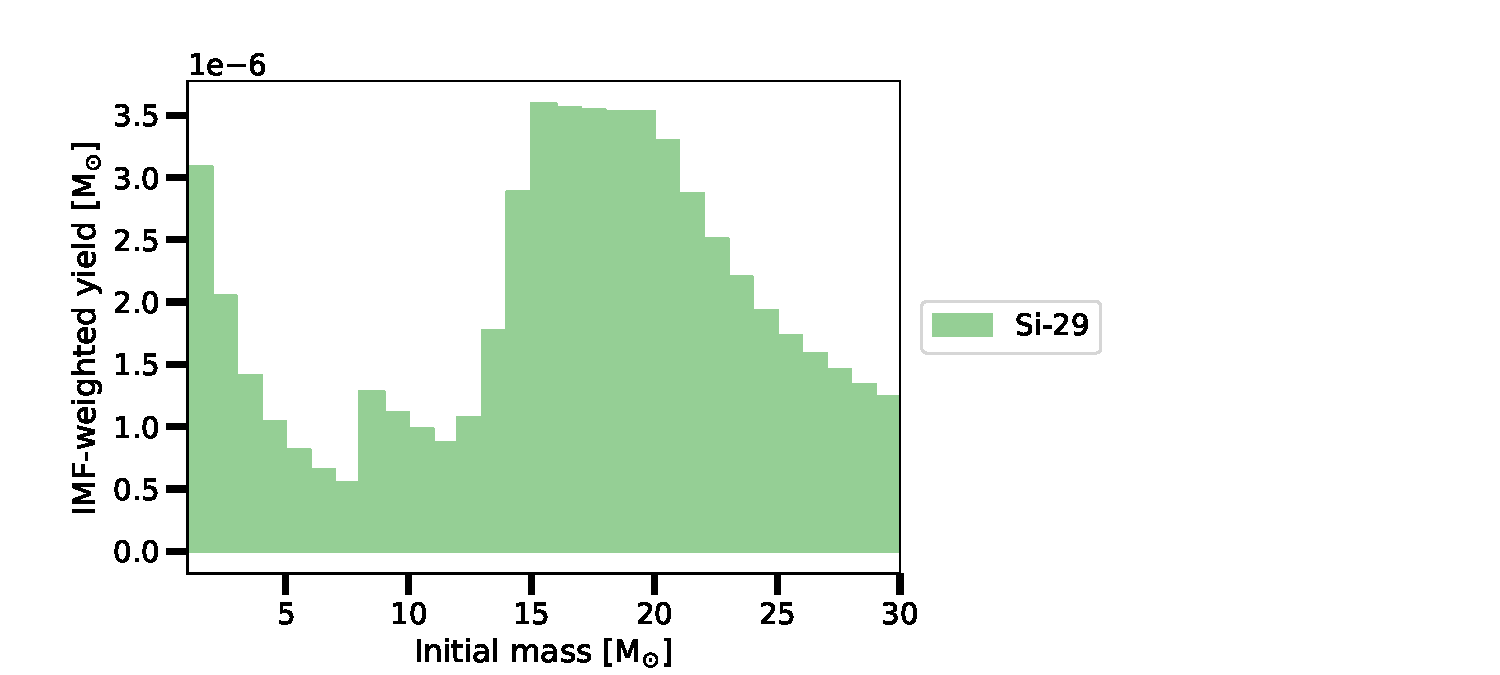
\includegraphics[width=\textwidth]{figs/Si-29_Z=0.02_yield.pdf}
        \caption{IMF-weighted stellar nucleosynthesis yield of \iso{29}{Si}.}
    \end{subfigure}
    \centering
    \begin{subfigure}[c]{0.6\textwidth}
        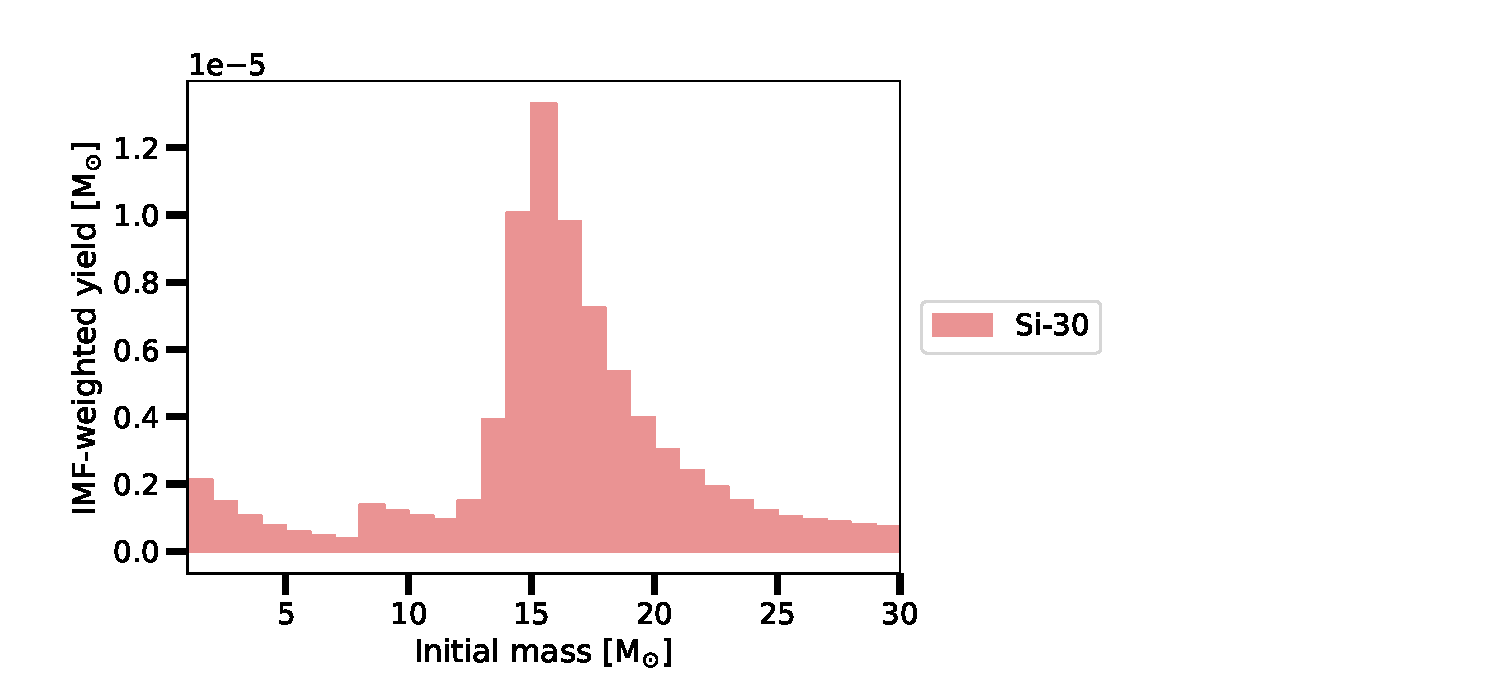
\includegraphics[width=\textwidth]{figs/Si-30_Z=0.02_yield.pdf}
        \caption{IMF-weighted stellar nucleosynthesis yield of \iso{30}{Si}.}
    \end{subfigure}
    \caption{IMF-weighted stellar nucleosynthesis yield of Si isotopes for stellar models with initial metallicity $Z=0.02$. The yields for the stellar model with initial mass $M_{ZAMS}/\msun = 1, 1.65, 2, 3, 4, 5, 6, 7, 12, 15, 20, 25$ are given by the NuGrid yield set (\citealt{Ritter_2018}). The yields for stars with a different initial mass are calculated using linear interpolation. The plots show that stars with initial mass $15\leq M_{ZAM}/\msun \leq 20$ are the major contributors of Si production when compared with other stars with the same initial metallicity $Z=0.02$.}
    \label{fig:imf_yield_0.02}
\end{figure}

\begin{figure}[H]
    \begin{subfigure}[c]{0.6\textwidth}
        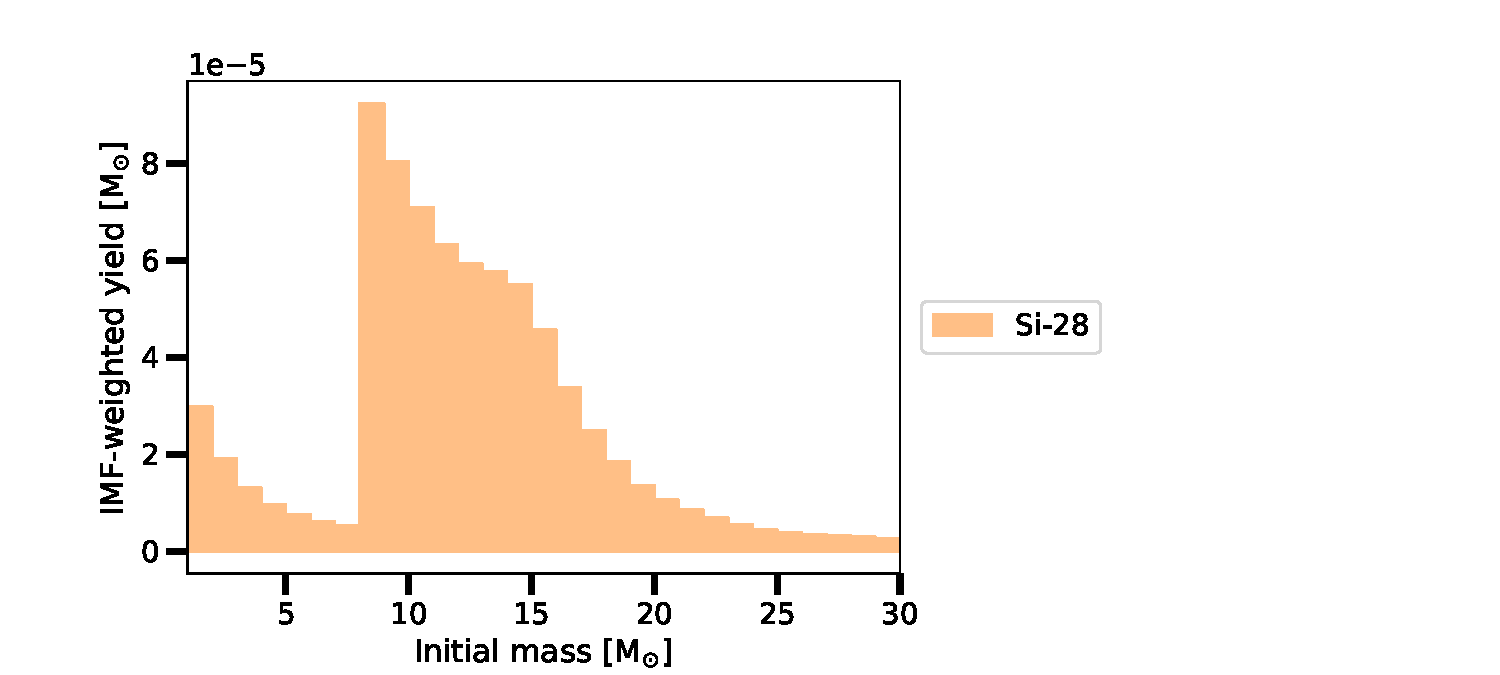
\includegraphics[width=\textwidth]{figs/Si-28_Z=0.01_yield.pdf}
        \caption{IMF-weighted stellar nucleosynthesis yield of \iso{28}{Si}.}
    \end{subfigure}
    \begin{subfigure}[c]{0.6\textwidth}
        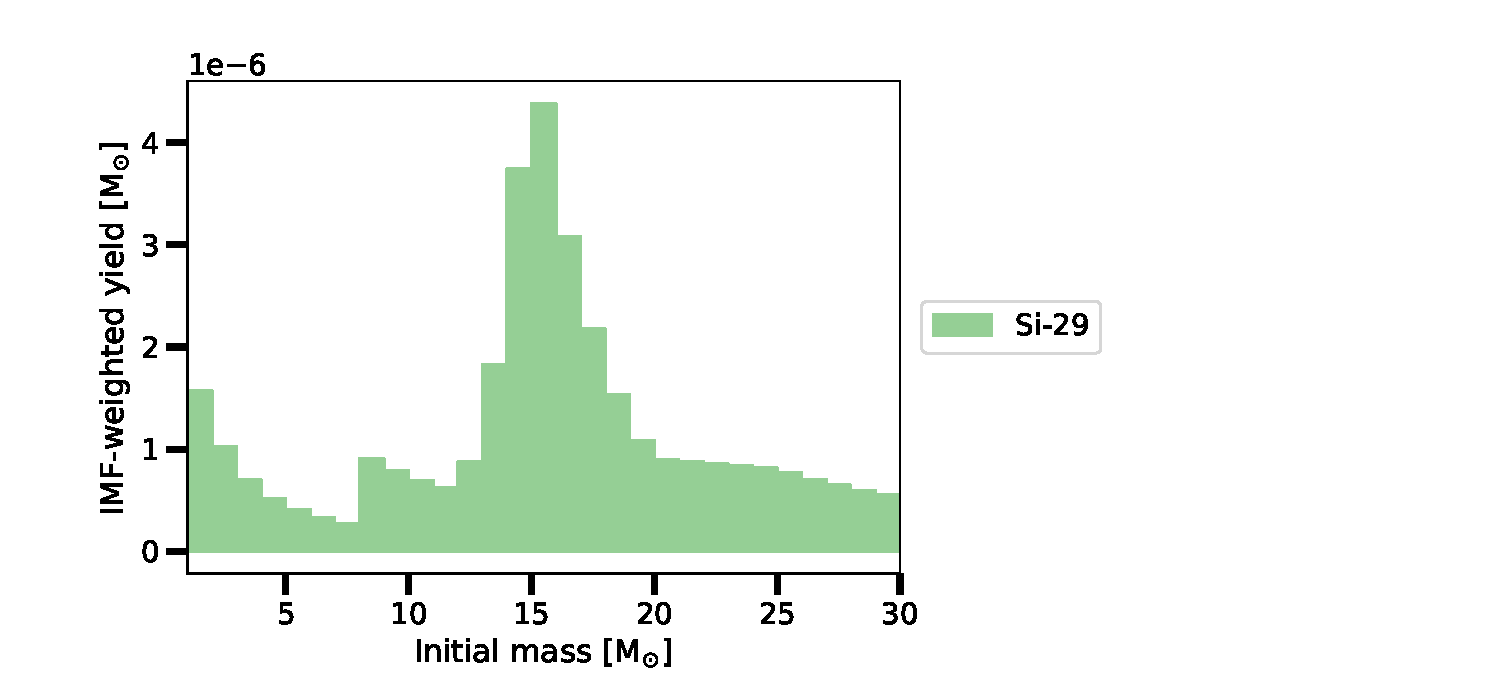
\includegraphics[width=\textwidth]{figs/Si-29_Z=0.01_yield.pdf}
        \caption{IMF-weighted stellar nucleosynthesis yield of \iso{29}{Si}.}
    \end{subfigure}
    \centering
    \begin{subfigure}[c]{0.6\textwidth}
        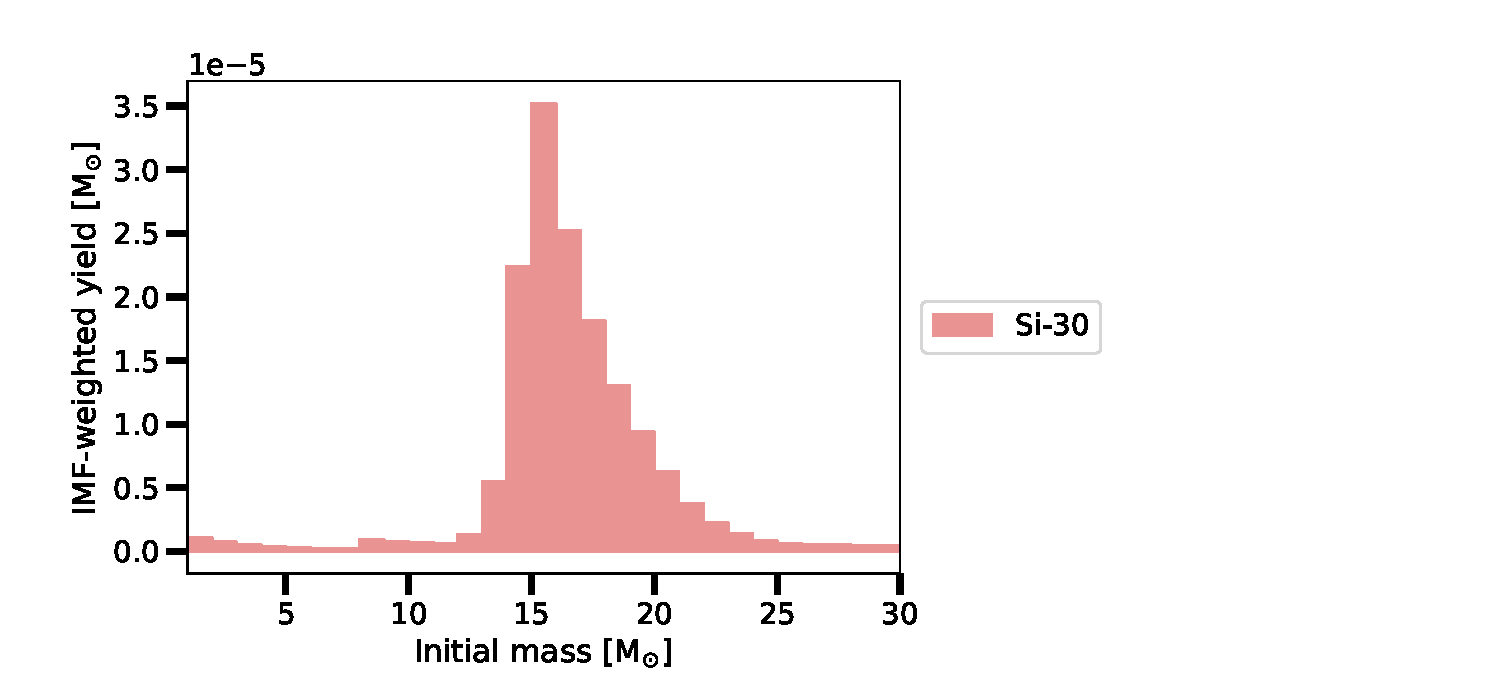
\includegraphics[width=\textwidth]{figs/Si-30_Z=0.01_yield.pdf}
        \caption{IMF-weighted stellar nucleosynthesis yield of \iso{30}{Si}.}
    \end{subfigure}
    \caption{IMF-weighted stellar nucleosynthesis yield of Si isotopes for stellar models with initial metallicity $Z=0.01$. The plots show that stars with initial mass $15\leq M_{ZAM}/\msun \leq 20$ are the most important source of \iso{29,\, 30}{Si} compared to other stars with the same metallicity $Z=0.01$.}
    \label{fig:imf_yield_0.01}
\end{figure}



\section{Main Silicon Production Regions in Massive Stars} \label{si_region}
After determining the stars responsible for silicon production in the galaxy, I determine the main silicon production regions in those stars. \cite{Curtis_2018} shows that \iso{29}{Si} and \iso{30}{Si} are formed during the explosive oxygen burning in massive stars. Therefore, this work will focus on the explosive nucleosynthesis of stars with initial mass $15 \leq M_{ZAM}/\msun \leq 20$, in particular, NuGrid models with $M_{ZAM}/\msun = 15, 20$. I find the silicon production regions in those stars by comparing the pre-supernova and post-supernova isotopic abundances. The identified mass coordinate ranges for the silicon production region are shown in Table \ref{tab:massrange}. The main reactions affecting the production and destruction of silicon isotopes in these regions are shown in Table \ref{tab:si_reaction}.

\begin{table}[H]
    \centering
    \caption{Mass coordinate range for the silicon production regions in different stellar models with initial mass $M_{ZAM}$ and initial metallicity $Z$.}
\begin{tabular}{c c c}
        \hline
          Initial Mass $M_{ZAM}$ ($\msun$) &    Initial Metallicity $Z$& Mass Coordinate Range (\msun)\\
        \hline
        % 12   & 0.02 & 1.96\,-\,2.45\\
        % 12   & 0.01 & 2.12\,-\,2.81\\
        15   & 0.02 & 2.99\,-\,3.70\\
        15   & 0.01 & 3.13\,-\,4.19\\
        20   & 0.02 & 4.52\,-\,6.36\\
        20   & 0.01 & 4.97\,-\,6.34\\
        \hline
    \end{tabular}
    \label{tab:massrange}
\end{table}

\begin{table}[H]
    \centering
    \caption{Main silicon production reactions and the upper ($U^{\rm hi}$) and lower ($U^{\rm lo}$) limits of their variation factors}
\begin{tabular}{c c c}
    \hline
      Reaction  & $U^{\rm hi}$ & $U^{\rm lo}$\\
    \hline
    \iso{28}{Si}$(n, \gamma)$\iso{29}{Si}& 1.18 & 0.82\\
    \iso{29}{Si}$(n, \gamma)$\iso{30}{Si}& 1.20 & 0.80\\
    \iso{30}{Si}$(n, \gamma)$\iso{31}{Si}& 1.36 & 0.64\\
    \iso{25}{Mg}$(\alpha, n)$\iso{28}{Si}& 2.00 & 0.10\\
    \iso{26}{Mg}$(\alpha, n)$\iso{29}{Si}& 2.00 & 0.10\\
    \iso{33}{S}$(n, \alpha)$\iso{30}{Si}& 2.00 & 0.10\\
    \hline
    \end{tabular}
    \label{tab:si_reaction}
\end{table}



% \subsection{Stellar Models with Initial Mass $M/\msun = 12$}

% Figure \ref{fig:m12z02} shows the comparison between pre-supernova and post-supernova isotopic abundances for stellar model with initial mass $M/\msun =12$ and initial metallicity $Z=0.02$. We see that between $M/\msun = 1.96$ and $M/\msun = 2.45$, the post-supernova \iso{29}{Si} and \iso{30}{Si} abundance are higher than the pre-supernova abundance. The pre-supernova \iso{29, 30}{Si} abundance is at the order of $10^{-5}$ while the post-supernova \iso{29,\, 30}{Si} abundance increase to up to $10^{-2}$. This increase shows that the heavy Si isotopes are produced in this region during the supernova explosion. We also see that the increase in silicon isotopic abundances corresponds to the decrease of \iso{16}{O} abundance which suggests that the identified region undergoes explosive oxygen burning. This result agrees with the result in \cite{Curtis_2018} and validates our approach.

% \begin{figure}[H]
%     \centering
%     \begin{subfigure}[c]{0.65\textwidth}
%         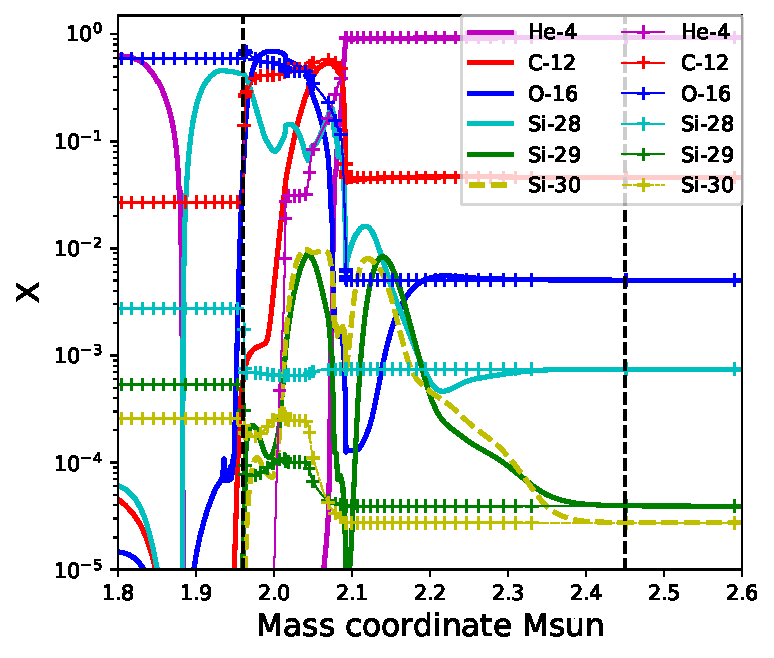
\includegraphics[width=\textwidth]{figs/120.02.pdf}
%     \end{subfigure}
%     % \begin{subfigure}[c]{0.5\textwidth}
%     %     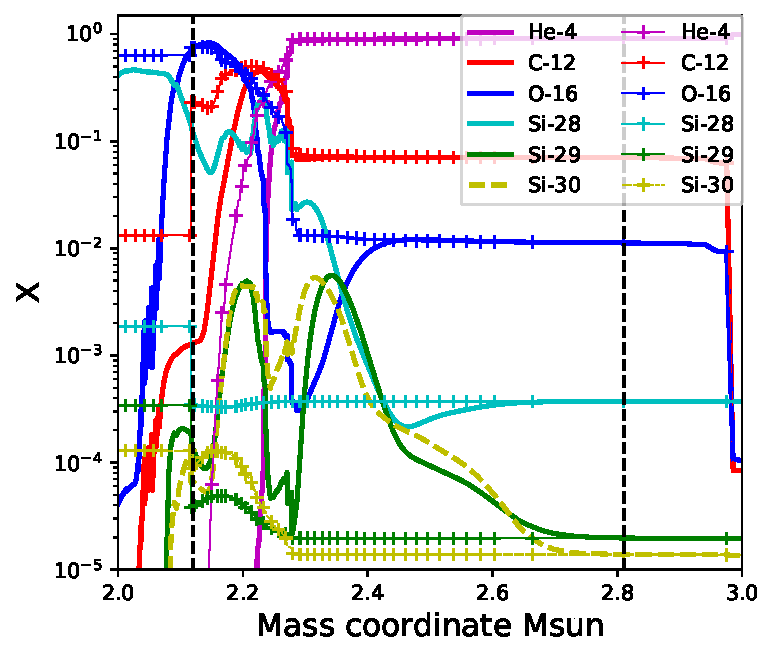
\includegraphics[width=\textwidth]{figs/120.01.pdf}
%     % \end{subfigure}
%     \caption{Comparison between pre-supernova and post-supernova isotopic abundances (expressed in mass fractions) for stellar model with initial mass $M/\msun =12$ and initial metallicity $Z=0.02$. The pre- and post- supernova abundance profiles for \iso{4}{He}, \iso{12}{C}, \iso{16}{O}, and \iso{28,\, 29,\, 30}{Si} are shown. The dotted lines represents the pre-supernova isotopic abundances. The solid lines represents the isotopic abundances immediately after CCSNe. The black dashed lines represent the ranges of mass coordinate that are responsible for silicon production in these stellar models. The black dashed lines are at mass coordinate $M/\msun = 1.96$ and $M/\msun = 2.45$.}
%     \label{fig:m12z02}
% \end{figure}

% \begin{figure}[H]
%     \centering
%     \begin{subfigure}[c]{0.65\textwidth}
%         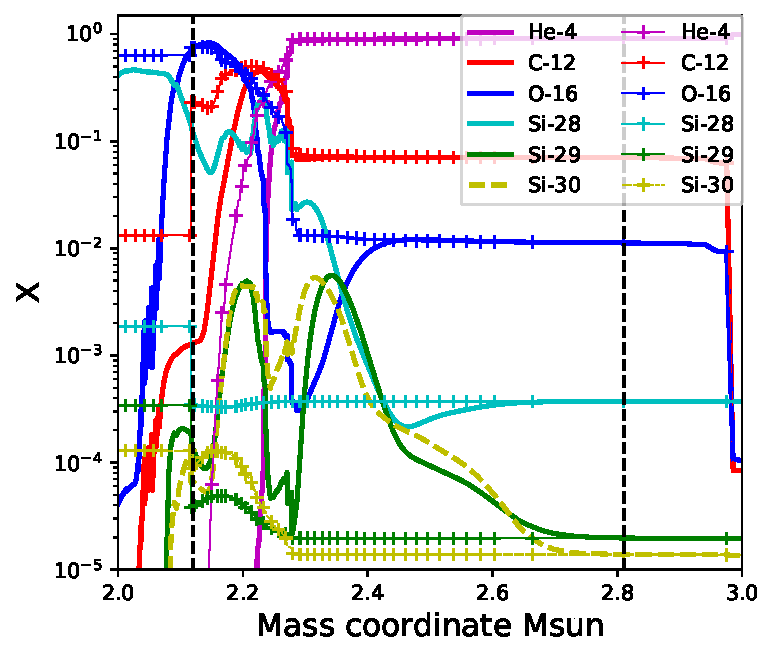
\includegraphics[width=\textwidth]{figs/120.01.pdf}
%     \end{subfigure}
%     \caption{Comparison between pre-supernova and post-supernova isotopic abundances for stellar model with initial mass $M/\msun =12$ and initial metallicity $Z=0.01$ with the same symbols used in Figure \ref{fig:m12z02}. The black dashed lines are at mass coordinate $M/\msun = 2.12$ and $M/\msun = 2.81$.}
%     \label{fig:m12z01}
% \end{figure}

% Figure \ref{fig:m12z01} shows the comparison between pre-supernova and post-supernova isotopic abundances for stellar model with initial mass $M/\msun =12$ and initial metallicity $Z=0.01$. We see a similar increase in the post-supernova \iso{29,\, 30}{Si} abundance as shown in Figure \ref{fig:m12z02} between $M/\msun = 2.12$ and $M/\msun = 2.81$. The pre-supernova \iso{29, 30}{Si} composition is at the order of $10^{-5}$ while the post-supernova \iso{29, 30}{Si} composition increase to up to $5\times 10^{-3}$. This region also undergoes explosive oxygen burning as suggested by the decrease in \iso{16}{O}

\subsection[Stellar Models with Initial Mass $M_{ZAM}/\msun = 15$]{Stellar Models with Initial Mass $\mathbf{M_{ZAM}/\msun = 15}$}
Figures \ref{fig:m15z02} and \ref{fig:m15z01} present a comparison between pre-supernova and post-supernova isotopic abundances for two stellar models with an initial mass of $M_{ZAM}/\msun =15$, and initial metallicities of $Z=0.02$ and $Z=0.01$, respectively. In the $Z=0.02$ model shown in Figure \ref{fig:m15z02}, for the mass coordinate range $M/\msun = 2.99 - 3.70$, the pre-supernova \iso{29, 30}{Si} mass fractions are about $10^{-5}$, whereas the post-supernova \iso{29, 30}{Si} mass fractions increase to $3\times 10^{-3}$ for \iso{29}{Si} and $1\times 10^{-3}$ for \iso{30}{Si}. A decrease in the \iso{16}{O} mass fraction is observed, indicating explosive oxygen-burning conditions in the identified region. Figure \ref{fig:m15z02} shows that Si isotopes are produced in explosive oxygen burning region at mass coordinate $M/\msun = 2.99-3.70$ in stellar model with $M_{ZAM}/\msun =15$ and $Z=0.02$. In the $Z=0.01$ model shown in Figure \ref{fig:m15z01}, the pre-supernova \iso{29, 30}{Si} mass fractionss are around $10^{-5}$ for the mass range $M/\msun = 3.13 - 4.19$, whereas the post-supernova \iso{29, 30}{Si} mass fractions increase to $1\times 10^{-2}$ for \iso{29}{Si} and $4\times 10^{-3}$ for \iso{30}{Si}. I also see a decrease in the \iso{16}{O} mass fraction, which suggests the identified region undergoes explosive oxygen burning during CCSNe. Figure \ref{fig:m15z01} shows that Si isotopes are produced in explosive oxygen burning region at mass coordinate $M/\msun = 3.13-4.19$ in stellar model with $M_{ZAM}/\msun =15$ and $Z=0.01$. These results show that Si isotopes are produced during explosive oxygen burning in stellar models with initial mass $M_{ZAM}/\msun =15$. 

\begin{figure}[H]
    \centering
    \begin{subfigure}[c]{0.6\textwidth}
        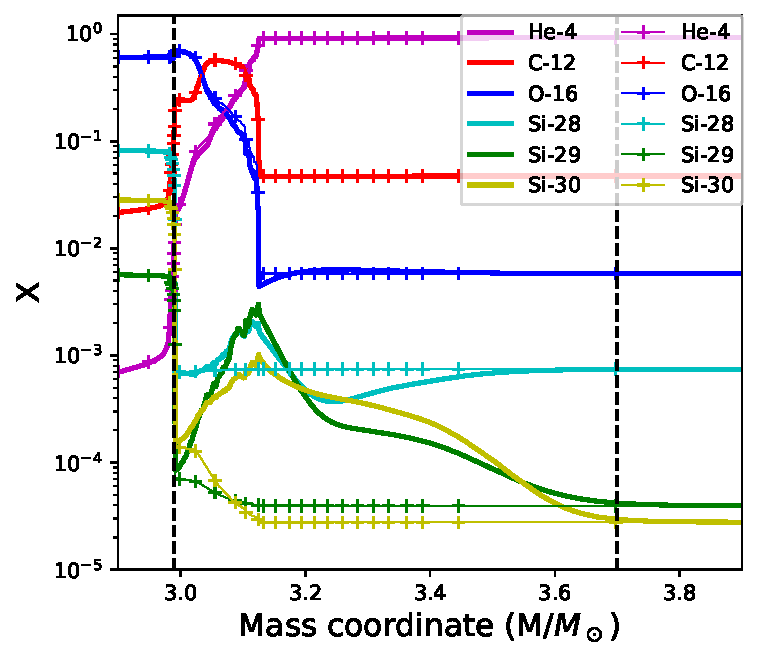
\includegraphics[width=\textwidth]{figs/150.02.pdf}
    \end{subfigure}
    \caption{Comparison between pre-supernova and post-supernova isotopic abundances (expressed in mass fractions) for the stellar model with initial mass $M_{ZAM}/\msun =15$ and initial metallicity $Z=0.02$. The pre- and post- supernova abundance profiles for \iso{4}{He}, \iso{12}{C}, \iso{16}{O}, and \iso{28,\, 29,\, 30}{Si} are shown. Thin lines with plus markers represent the pre-supernova isotopic abundances. The solid lines represent the isotopic abundances immediately after the explosion. The black dashed lines represent the ranges of mass coordinates that are responsible for silicon production in these stellar models. The black dashed lines are at mass coordinate $M/\msun = 2.99$ and $M/\msun = 3.70$. This figure shows that Si isotopes are produced in explosive oxygen burning region at mass coordinate $M/\msun = 2.99-3.70$ in stellar model with $M_{ZAM}/\msun =15$ and $Z=0.02$.}
    \label{fig:m15z02}
\end{figure}

\begin{figure}[H]
    \centering
    \begin{subfigure}[c]{0.6\textwidth}
        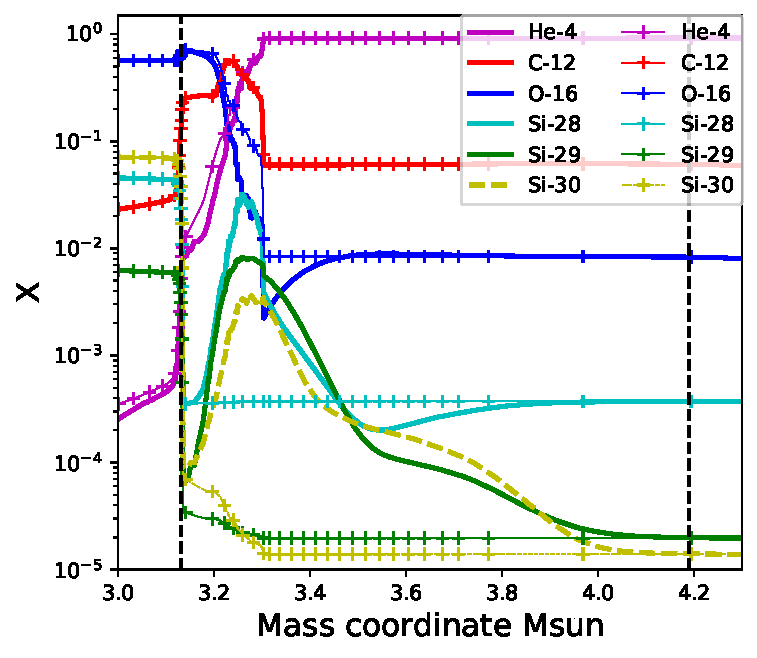
\includegraphics[width=\textwidth]{figs/150.01.pdf}
    \end{subfigure}
    \caption{Comparison between pre-supernova and post-supernova isotopic abundances (mass fraction) for the stellar model with initial mass $M_{ZAM}/\msun =15$ and initial metallicity $Z=0.01$ with the same symbols used in Figure \ref{fig:m15z02}. The black dashed lines are at mass coordinate $M/\msun = 3.13$ and $M/\msun = 4.19$. This figure shows that Si isotopes are produced in explosive oxygen burning region at mass coordinate $M/\msun = 3.13-4.19$ in stellar model with $M_{ZAM}/\msun =15$ and $Z=0.01$}
    \label{fig:m15z01}
\end{figure}



\subsection[Stellar Models with Initial Mass $M_{ZAM}/\msun = 20$]{Stellar Models with Initial Mass $\mathbf{M_{ZAM}/\msun = 20}$}

Figures \ref{fig:m20z02} and \ref{fig:m20z01} present a comparison between pre-supernova and post-supernova isotopic abundances for two stellar models with an initial mass of $M_{ZAM}/\msun =20$, and initial metallicities of $Z=0.02$ and $Z=0.01$, respectively. In the $Z=0.02$ model shown in Figure \ref{fig:m20z02}, the pre-supernova \iso{29, 30}{Si} mass fractions are about $10^{-5}$, while the post-supernova \iso{29, 30}{Si} mass fractions increase up to $10^{-2}$ between $M/\msun = 4.52 - 6.36$. The decrease in the \iso{16}{O} mass fraction suggests that the silicon isotopes are created during explosive oxygen burning in this stellar model. Figure \ref{fig:m20z02} shows that Si isotopes are produced in explosive oxygen burning region at mass coordinate $M/\msun = 4.52-6.36$ in stellar model with $M_{ZAM}/\msun =20$ and $Z=0.02$. In the $Z=0.01$ model shown in Figure \ref{fig:m20z01}, the pre-supernova \iso{29, 30}{Si} mass fractions are about $10^{-5}$, while the post-supernova \iso{29, 30}{Si} mass fractions increase to $5\time 10^{-3}$ for \iso{29}{Si} and $1\times 10^{-3}$ for \iso{30}{Si} between $M/\msun = 4.97 - 6.34$. The decrease in the \iso{16}{O} mass fraction suggests that the silicon isotopes are created during explosive oxygen burning in this stellar model. Figure \ref{fig:m20z01} shows that Si isotopes are produced in explosive oxygen burning region at mass coordinate $M/\msun = 4.97-6.34$ in stellar model with $M_{ZAM}/\msun =20$ and $Z=0.01$. These results show that Si isotopes are produced during explosive oxygen burning in stellar models with initial mass $M_{ZAM}/\msun =20$. 

\begin{figure}[H]
    \centering
    \begin{subfigure}[c]{0.6\textwidth}
        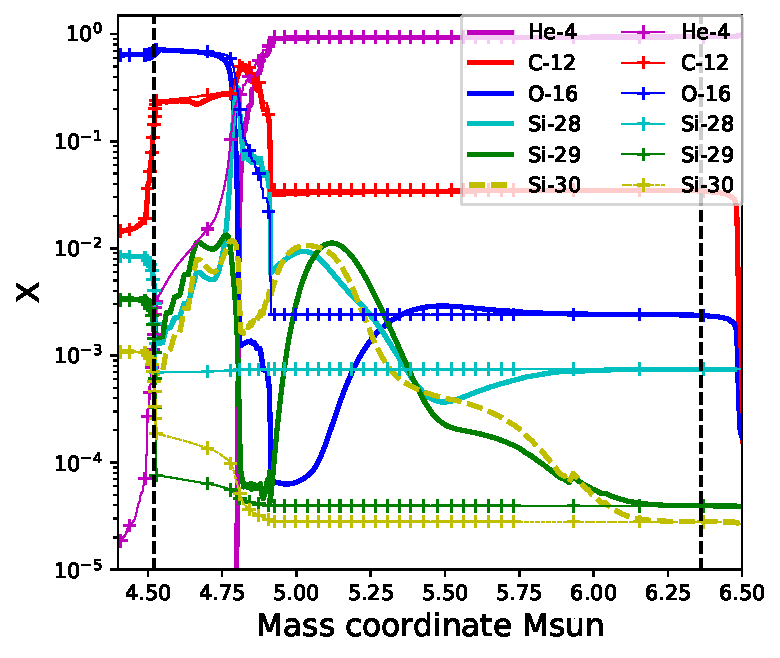
\includegraphics[width=\textwidth]{figs/200.02.pdf}
    \end{subfigure}
    \caption{Comparison between pre-supernova and post-supernova isotopic abundances (mass fraction) for the stellar model with initial mass $M_{ZAM}/\msun =20$ and initial metallicity $Z=0.02$ with the same symbols used in Figure \ref{fig:m15z02}. The black dashed lines are at mass coordinate $M/\msun = 4.52$ and $M/\msun = 6.36$. This figure shows that Si isotopes are produced in explosive oxygen burning region at mass coordinate $M/\msun = 4.52-6.36$ in stellar model with $M_{ZAM}/\msun =20$ and $Z=0.02$.}
    \label{fig:m20z02}
\end{figure}

\begin{figure}[H]
    \centering
    \begin{subfigure}[c]{0.6\textwidth}
        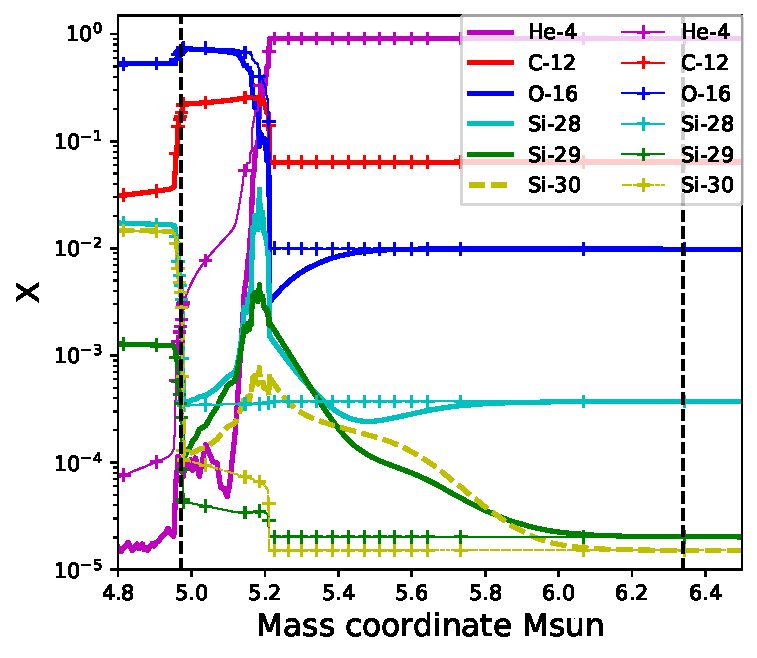
\includegraphics[width=\textwidth]{figs/200.01.pdf}
    \end{subfigure}
    \caption{Comparison between pre-supernova and post-supernova isotopic abundances (mass fractions) for the stellar model with initial mass $M_{ZAM}/\msun =15$ and initial metallicity $Z=0.01$ with the same symbols used in Figure \ref{fig:m15z02}. The black dashed lines are at mass coordinate $M/\msun = 4.97$ and $M/\msun = 6.34$. This figure shows that Si isotopes are produced in explosive oxygen burning region at mass coordinate $M/\msun = 4.97-6.34$ in stellar model with $M_{ZAM}/\msun =20$ and $Z=0.01$.}
    \label{fig:m20z01}
\end{figure}



\subsection{Main Silicon Production Reactions}
In the identified regions, I find six major reactions for the production and destruction of silicon isotopes. These reactions and the upper and lower limits of their variation factors is shown in Table \ref{tab:si_reaction}. For the $(n,\gamma)$ reactions, their upper and lower limits are determined using experimental uncertainties given on Karlsruhe Astrophysical Database of Nucleosynthesis in Stars (KADoNiS).\footnote{https://kadonis.org} For other reactions, I use the theoretical upper and lower limits given in Table \ref{tab:rate}.


% \section{Nucleosynthesis with Increase \iso{26}{Mg}$(\alpha, n)$\iso{29}{Mg} Rate}


\chapter{Monte Carlo Result} \label{mc_result}
For the Monte Carlo simulation, I take 20 trajectories equally spaced in their mass coordinate from each of the stellar regions in Table \ref{tab:massrange}. I take 100 different sets of rate variation factors following the recipe in Section \ref{mc} and the upper and lower limits in Table \ref{tab:si_reaction}. Section \ref{nucleo_result} shows the result for each stellar region. Section \ref{yield_result} shows the integrated stellar yield for different stellar models. Section \ref{gce_result} shows the Monte Carlo results for the GCE of silicon isotopes in comparison with the mainstream grain measurements. 

\section{Nucleosynthesis Result} \label{nucleo_result}

\subsection[Stellar Models with Initial Mass $M_{ZAM}/\msun = 15$]{Stellar Models with Initial Mass $\mathbf{M_{ZAM}/\msun = 15}$}
Figures \ref{fig:m15z02_region} and \ref{fig:m15z01_region} present the variation in silicon isotopic abundances immediately after supernova explosion for two stellar models with an initial mass of $M_{ZAM}/\msun =15$, and initial metallicities of $Z=0.02$ and $Z=0.01$, respectively. The upper and lower limits are derived from the Monte Carlos simulation of the nucleosynthesis calculation. In the $Z=0.02$ model shown in Figure \ref{fig:m15z02_region}, the \iso{29, \, 30}{Si} abundances are affected by the nuclear uncertainties while the \iso{28}{Si} abundances remain largely unchanged. In particular, the nuclear uncertainties have the largest effect on the \iso{29}{Si} abundance with an increase up to 73\% and a decrease up to 74\% in the \iso{29}{Si} mass fraction. The maximum increase in the \iso{30}{Si} mass fraction is 45\%. The maximum decrease in the \iso{30}{Si} mass fraction is 35\%. The maximum increase in the \iso{28}{Si} mass fraction is 16\%. The maximum decrease in the \iso{28}{Si} mass fraction is 13\%. In the $Z=0.01$ model shown in Figure \ref{fig:m15z01_region}, similar to the $Z=0.02$ model, the \iso{29, \, 30}{Si} abundances are affected by the nuclear uncertainties while the \iso{28}{Si} abundances remain largely unchanged. In particular, the nuclear uncertainties have the largest effect on the \iso{29}{Si} abundance with an increase up to 74\% and a decrease up to 75\% in the \iso{29}{Si} mass fraction. The maximum increase in the \iso{30}{Si} mass fraction is 52\%. The maximum decrease in the \iso{30}{Si} mass fraction is 44\%. The maximum increase in the \iso{28}{Si} mass fraction is 15\%. The maximum decrease in the \iso{28}{Si} mass fraction is 12\%. Figure \ref{fig:m15z02_region} and \ref{fig:m15z01_region} show that nuclear uncertainties do affect the nucleosynthesis of heavy Si isotopes, \iso{29,\, 30}{Si}, in stellar models with initial mass $M_{ZAM}/\msun =15$ at initial metallicity $Z=0.02,\, 0.01$.


\begin{figure}[H]
    \centering
    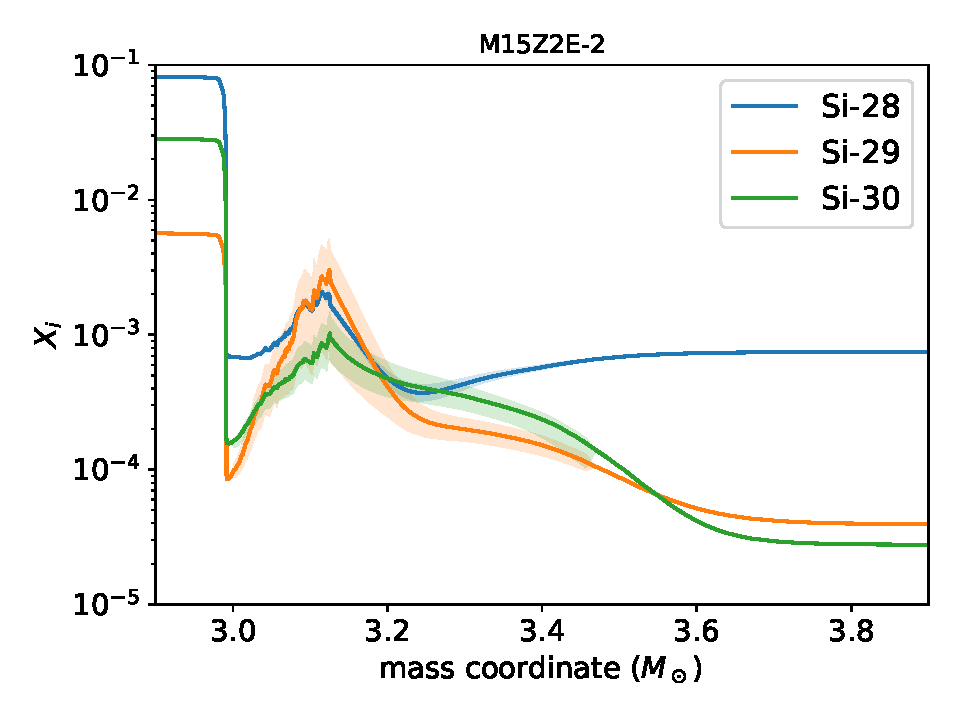
\includegraphics[width=0.7\textwidth]{figs/M15Z2E-2_mcresult.pdf}
    \caption{Monte Carlo result of post-supernova silicon isotopic abundances (mass fraction) in the stellar model with initial mass $M_{ZAM}/\msun =15$ and initial metallicity $Z=0.02$. The blue, orange, and green lines represent the mass fraction of \iso{28}{Si}, \iso{29}{Si}, and \iso{30}{Si}, respectively. The solid line represents the mass fraction in the NuGrid model (\cite{Ritter_2018}). The shades represent the range of mass fractions derived from the Monte Carlo result. This plot shows that nuclear uncertainties do affect the nucleosynthesis of \iso{29,\, 30}{Si} in stellar model with $M_{ZAM}/\msun =15$, $Z=0.02$.}
    \label{fig:m15z02_region}
\end{figure}

\begin{figure}[H]
    \centering
    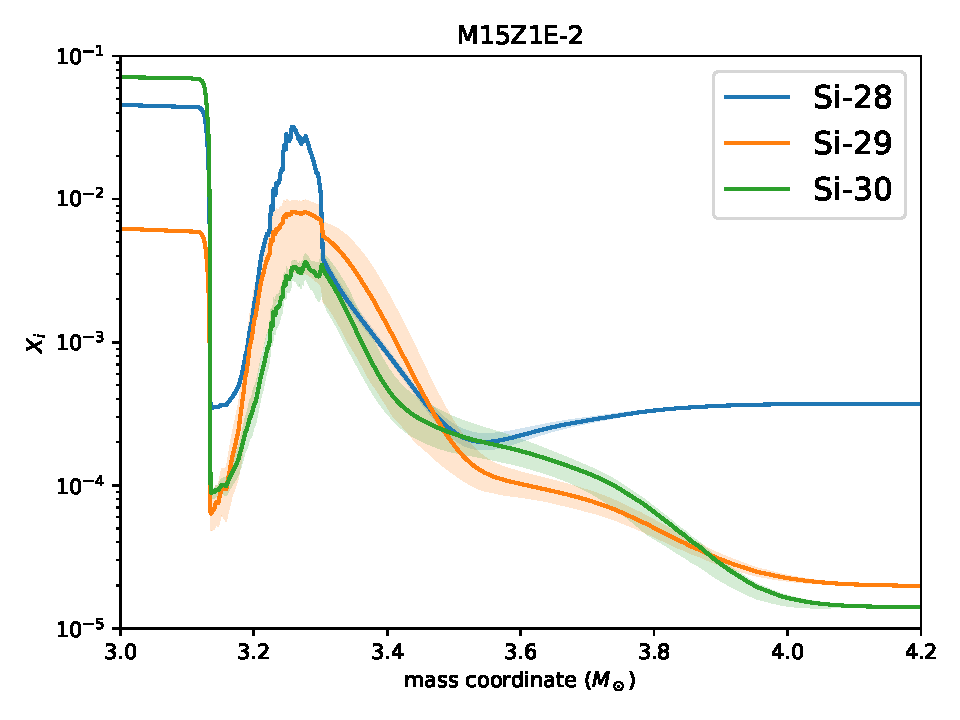
\includegraphics[width=0.7\textwidth]{figs/M15Z1E-2_mcresult.pdf}
    \caption{Monte Carlo result of post-supernova silicon isotopic abundances (mass fraction) in the stellar model with initial mass $M_{ZAM}/\msun =15$ and initial metallicity $Z=0.01$ with the same symbols used in Figure \ref{fig:m15z02_region}. This plot shows that nuclear uncertainties do affect the nucleosynthesis of \iso{29,\, 30}{Si} in stellar model with $M_{ZAM}/\msun =15$, $Z=0.01$.}
    \label{fig:m15z01_region}
\end{figure}


\subsection[Stellar Models with Initial Mass $M_{ZAM}/\msun = 20$]{Stellar Models with Initial Mass $\mathbf{M_{ZAM}/\msun = 20}$}
Figures \ref{fig:m20z02_region} and \ref{fig:m20z01_region} present the variation in silicon isotopic abundances immediately after supernova explosion for two stellar models with an initial mass of $M_{ZAM}/\msun =20$, and initial metallicities of $Z=0.02$ and $Z=0.01$, respectively. The upper and lower limits are derived from the Monte Carlos simulation of the nucleosynthesis calculation. In the $Z=0.02$ model shown in Figure \ref{fig:m20z02_region}, the \iso{29, \, 30}{Si} abundances are affected by the nuclear uncertainties while the \iso{28}{Si} abundances remain largely unchanged. In particular, the nuclear uncertainties have the largest effect on the \iso{29}{Si} abundances with an increase up to 82\% and a decrease up to 76\% in the \iso{29}{Si} mass fraction. The maximum increase in the \iso{30}{Si} mass fraction is 57\%. The maximum decrease in the \iso{30}{Si} mass fraction is 49\%. The maximum increase in the \iso{28}{Si} mass fraction is 19\%. The maximum decrease in the \iso{28}{Si} mass fraction is 14\%. In the $Z=0.01$ model shown in Figure \ref{fig:m20z01_region}, the \iso{29, \, 30}{Si} abundances are affected by the nuclear uncertainties while the \iso{28}{Si} abundances remain largely unchanged. In particular, the nuclear uncertainties have the largest effect on the \iso{29}{Si} abundances with an increase up to 76\% and a decrease up to 76\% in the \iso{29}{Si} mass fraction. The maximum increase in the \iso{30}{Si} mass fraction is 54\%. The maximum decrease in the \iso{30}{Si} mass fraction is 39\%. The maximum increase in the \iso{28}{Si} mass fraction is 13\%. The maximum decrease in the \iso{28}{Si} mass fraction is 11\%. Figure \ref{fig:m20z02_region} and \ref{fig:m20z01_region} show that nuclear uncertainties do affect the nucleosynthesis of heavy Si isotopes, \iso{29,\, 30}{Si}, in stellar models with initial mass $M_{ZAM}/\msun =20$ at initial metallicity $Z=0.02,\, 0.01$. 

\begin{figure}[H]
    \centering
    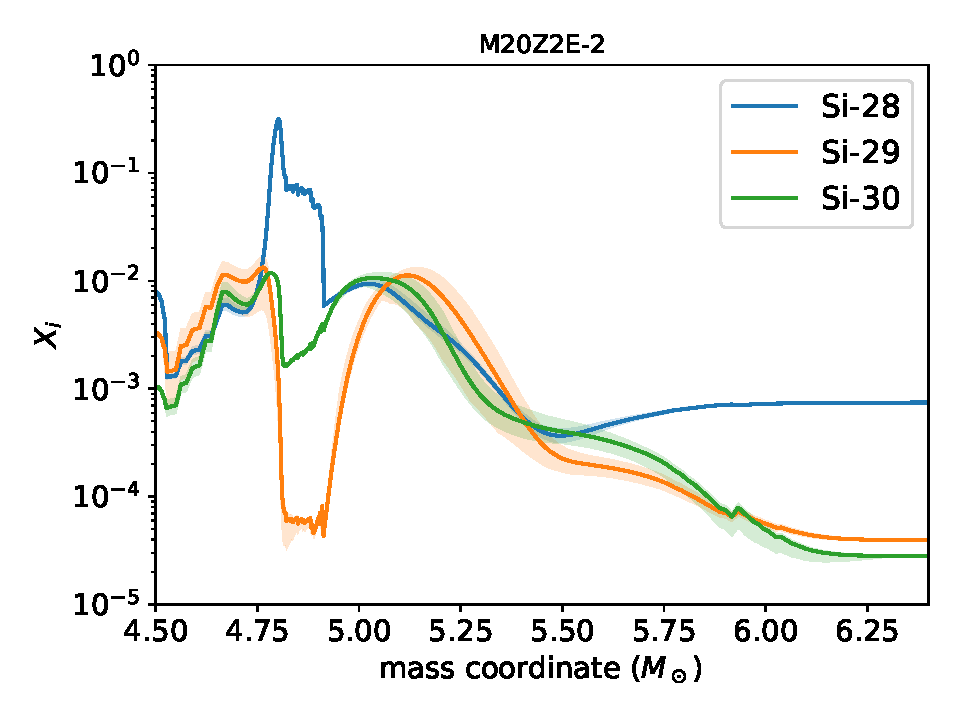
\includegraphics[width=0.7\textwidth]{figs/M20Z2E-2_mcresult.pdf}
    \caption{Monte Carlo result of post-supernova silicon isotopic abundances (mass fraction) in the stellar model with initial mass $M_{ZAM}/\msun =20$ and initial metallicity $Z=0.02$ with the same symbols used in Figure \ref{fig:m15z02_region}. This figure shows that nuclear uncertainties do affect the nucleosynthesis of heavy Si isotopes, \iso{29,\, 30}{Si}, in stellar models with initial mass $M_{ZAM}/\msun =20$ at initial metallicity $Z=0.02$.}
    \label{fig:m20z02_region}
\end{figure}


\begin{figure}[H]
    \centering
    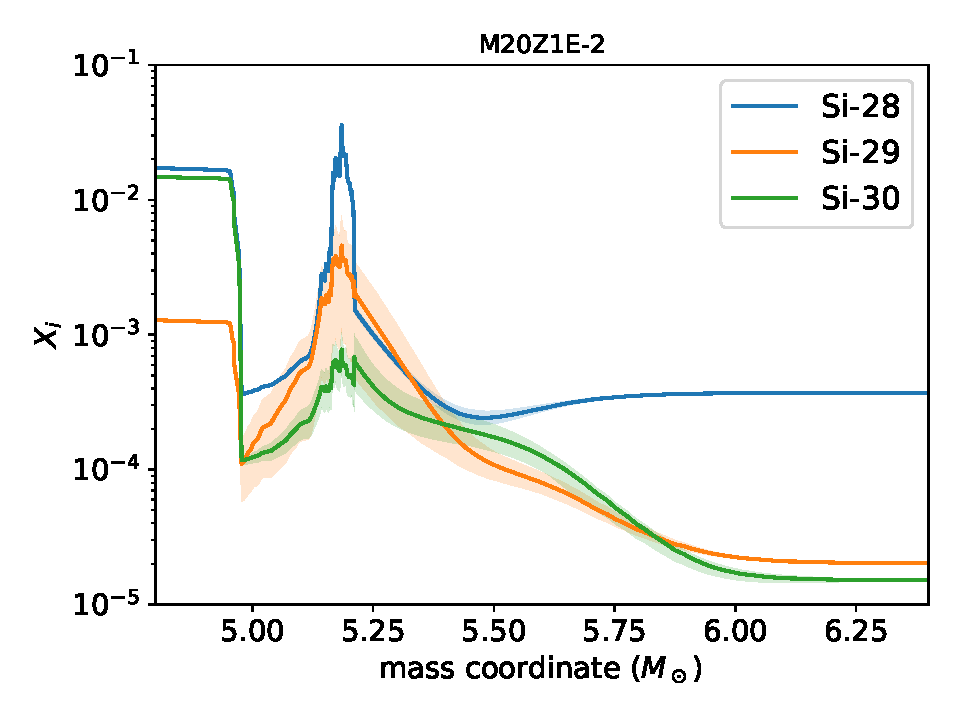
\includegraphics[width=0.7\textwidth]{figs/M20Z1E-2_mcresult.pdf}
    \caption{Monte Carlo result of post-supernova silicon isotopic abundances in the stellar model with initial mass $M_{ZAM}/\msun =20$ and initial metallicity $Z=0.01$ with the same symbols used in Figure \ref{fig:m15z02_region}. This figure shows that nuclear uncertainties do affect the nucleosynthesis of heavy Si isotopes, \iso{29,\, 30}{Si}, in stellar models with initial mass $M_{ZAM}/\msun =20$ at initial metallicity $Z=0.01$.}
    \label{fig:m20z01_region}
\end{figure}

\section{Stellar Nucleosynthesis Yields} \label{yield_result}

\subsection[Stellar Models with Initial Mass $M_{ZAM}/\msun = 15$]{Stellar Models with Initial Mass $\mathbf{M_{ZAM}/\msun = 15}$}

Figures \ref{fig:m15z02_yield} and \ref{fig:m15z01_yield} present the variation in the stellar nucleosynthesis yields of silicon isotopes for two stellar models with an initial mass of $M_{ZAM}/\msun =15$, and initial metallicities of $Z=0.02$ and $Z=0.01$, respectively. The variation factor $\eta$ is given by,
\begin{equation}
    \eta = \frac{X_{i}}{X^{0}_i},
\end{equation}
where $X_i$ is the modified yield, and $X^0_i$ is the yield given by the NuGrid yield sets. In the $Z=0.02$ model shown in Figure \ref{fig:m15z02_yield}, the \iso{29}{Si} yield is affected by the nuclear uncertainties while the \iso{28, \, 30}{Si} yields remain largely unchanged. In particular, for the \iso{29}{Si} yield, I see an increase up to $18.3\permil$ and a decrease up to $17.3\permil$. The maximum increase in the \iso{30}{Si} yield is $1.4\permil$. The maximum decrease in the \iso{30}{Si} yield is $1.3\permil$. The maximum increase in the \iso{28}{Si} yield is $0.2\permil$. The maximum decrease in the \iso{28}{Si} yield is $0.1\permil$. In the $Z=0.01$ model shown in Figure \ref{fig:m15z01_yield}, similar to the $Z=0.02$ model, the \iso{29}{Si} yield is affected by the nuclear uncertainties while the \iso{28, \, 30}{Si} yields remain largely unchanged. In particular, for the \iso{29}{Si} yields, I see an increase up to $32.9\permil$ and a decrease up to $59.5\permil$. The maximum increase in the \iso{30}{Si} yield is $1.3\permil$. The maximum decrease in the \iso{30}{Si} yield is $1.5\permil$. The maximum increase in the \iso{28}{Si} yield is $0.3\permil$. The maximum decrease in the \iso{28}{Si} yield is $0.3\permil$. Figure \ref{fig:m15z02_yield} and \ref{fig:m15z01_yield} show that the nuclear uncertainties have the largest impact on the \iso{29}{Si} yield while \iso{28,\, 30}{Si} yields remain largely unchanged by the nuclear uncertainties in stellar models with $M_{ZAM}/\msun =15$ at initial metallicity $Z=0.02,\, 0.01$. 



\begin{figure}[H]
    \centering
    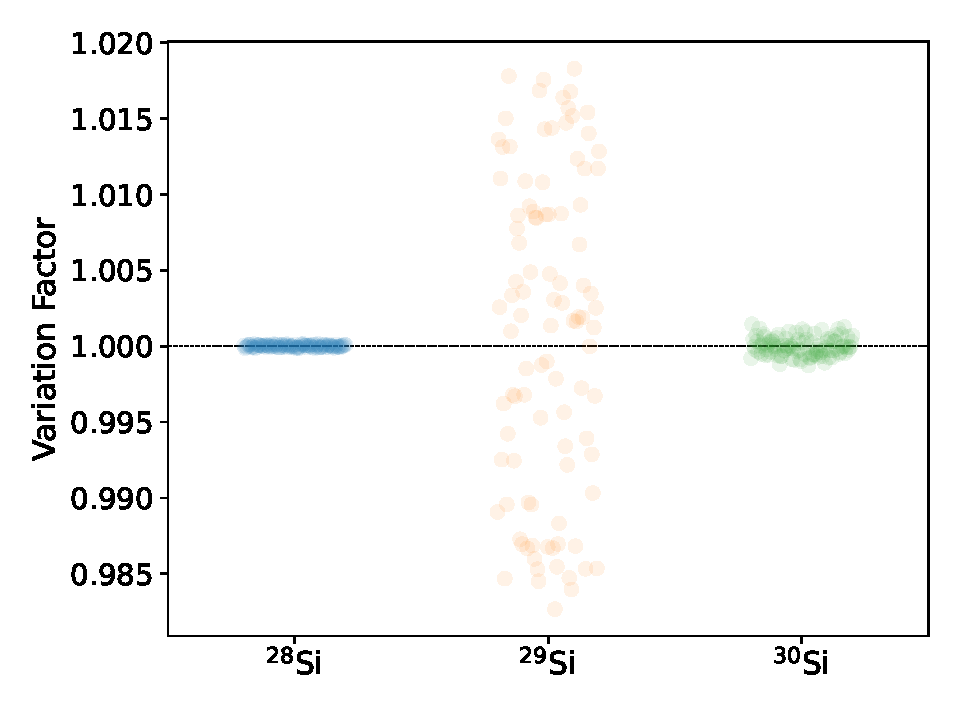
\includegraphics[width=0.7\textwidth]{figs/M15Z2E-2_mcyieldresult.pdf}
    \caption{Monte Carlo result of stellar nucleosynthesis yields in the stellar model with initial mass $M_{ZAM}/\msun =15$ and initial metallicity $Z=0.02$. The yields are represented as variation factors compared to the yields of the NuGrid model (\citealt{Ritter_2018}). The blue, orange, and green dots represent the variation factors of \iso{28}{Si}, \iso{29}{Si}, and \iso{30}{Si}, respectively. The black dotted line represents variation factor 1. This figure shows that the nuclear uncertainties have the largest impact on the \iso{29}{Si} yield while \iso{28,\, 30}{Si} yields remain largely unchanged by the nuclear uncertainties in the stellar model with $M_{ZAM}/\msun =15$, $Z=0.02$.}
    \label{fig:m15z02_yield}
\end{figure}

\begin{figure}[H]
    \centering
    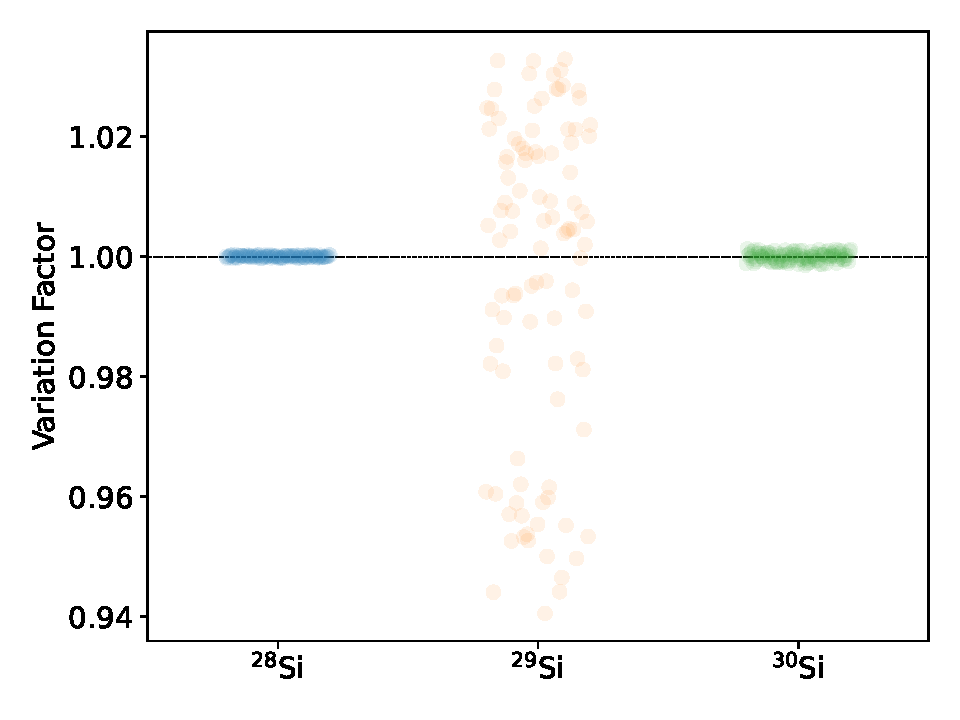
\includegraphics[width=0.7\textwidth]{figs/M15Z1E-2_mcyieldresult.pdf}
    \caption{Monte Carlo result of stellar nucleosynthesis yields in the stellar model with initial mass $M_{ZAM}/\msun =15$ and initial metallicity $Z=0.01$ with the same symbols used in Figure \ref{fig:m15z02_yield}. This figure shows that the nuclear uncertainties have the largest impact on the \iso{29}{Si} yield while \iso{28,\, 30}{Si} yields remain largely unchanged by the nuclear uncertainties in the stellar model with $M_{ZAM}/\msun =15$, $Z=0.02$.}
    \label{fig:m15z01_yield}
\end{figure}


\subsection[Stellar Models with Initial Mass $M_{ZAM}/\msun = 20$]{Stellar Models with Initial Mass $\mathbf{M_{ZAM}/\msun = 20}$}

Figures \ref{fig:m20z02_yield} and \ref{fig:m20z01_yield} present the variation in the stellar nucleosynthesis yields of silicon isotopes for two stellar models with an initial mass of $M_{ZAM}/\msun =20$, and initial metallicities of $Z=0.02$ and $Z=0.01$, respectively. In the $Z=0.02$ model shown in Figure \ref{fig:m20z02_yield}, the \iso{29, \, 30}{Si} yields are affected by the nuclear uncertainties while the \iso{28}{Si} yield remains largely unchanged. In particular, the nuclear uncertainties have the largest effect on the \iso{29}{Si} yield with an increase up to $84.6\permil$ and a decrease up to $146.2\permil$. The maximum increase in the \iso{30}{Si} yield is $46.4\permil$. The maximum decrease in the \iso{30}{Si} yield is $60.5\permil$. The maximum increase in the \iso{28}{Si} yield is $4.5\permil$. The maximum decrease in the \iso{28}{Si} yield is $2.7\permil$. In the $Z=0.01$ model shown in Figure \ref{fig:m20z01_yield}, the \iso{29}{Si} yield is affected by the nuclear uncertainties while the \iso{29, \, 30}{Si} yields remain largely unchanged. In particular, for the \iso{29}{Si} yield, I see an increase up to $75.5\permil$ and a decrease up to $78.0\permil$. The maximum increase in the \iso{30}{Si} yield is $1.5\permil$. The maximum decrease in the \iso{30}{Si} yield is $1.3\permil$. The maximum increase in the \iso{28}{Si} yield is $0.5\permil$. The maximum decrease in the \iso{28}{Si} yield is $0.5\permil$. The result shown by Figure \ref{fig:m20z02} suggests that the nuclear uncertainties affect \iso{29,\, 30}{Si} yield while the \iso{28}{Si} yields remain largely unchanged by the nuclear uncertainties in stellar model with $M_{ZAM}/\msun =20$, $Z=0.02$. The result shown by Figure \ref{fig:m20z01_yield} suggests that nuclear uncertainties have the largest impact on the \iso{29}{Si} yield while \iso{28,\, 30}{Si} yields remain largely unchanged in stellar model with $M_{ZAM}/\msun =20$, $Z=0.01$.
\begin{figure}[H]
    \centering
    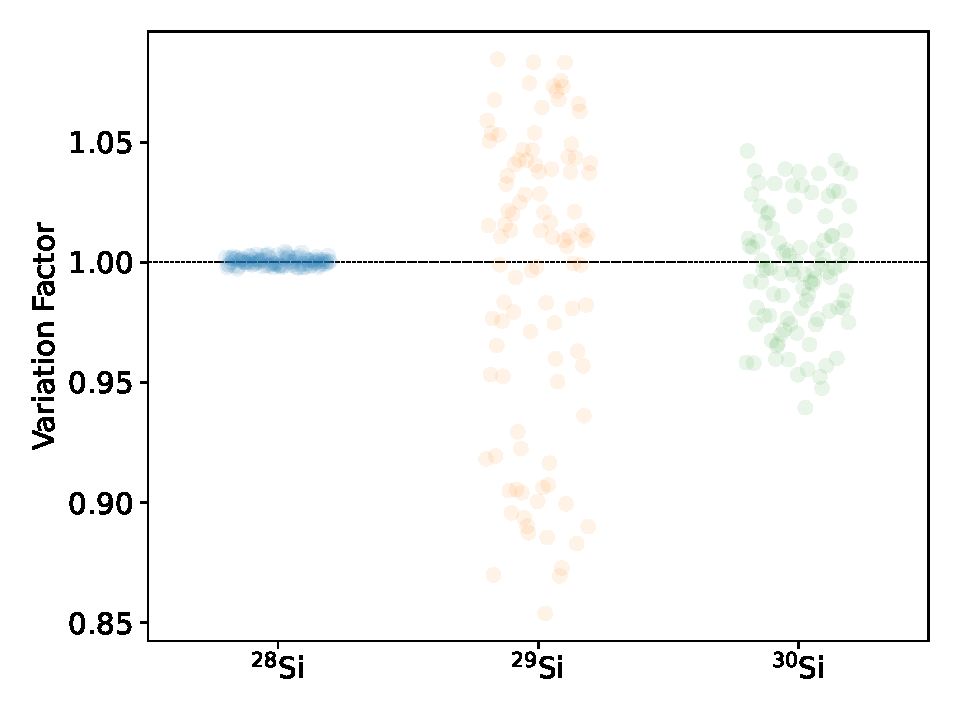
\includegraphics[width=0.7\textwidth]{figs/M20Z2E-2_mcyieldresult.pdf}
    \caption{Monte Carlo result of stellar nucleosynthesis yields in the stellar model with initial mass $M_{ZAM}/\msun =20$ and initial metallicity $Z=0.02$ with the same symbols used in Figure \ref{fig:m15z02_yield}. This figure shows that the nuclear uncertainties affect \iso{29,\, 30}{Si} yield while the \iso{28}{Si} yields remain largely unchanged by the nuclear uncertainties in the stellar model with $M_{ZAM}/\msun =20$, $Z=0.02$.}
    \label{fig:m20z02_yield}
\end{figure}

\begin{figure}[H]
    \centering
    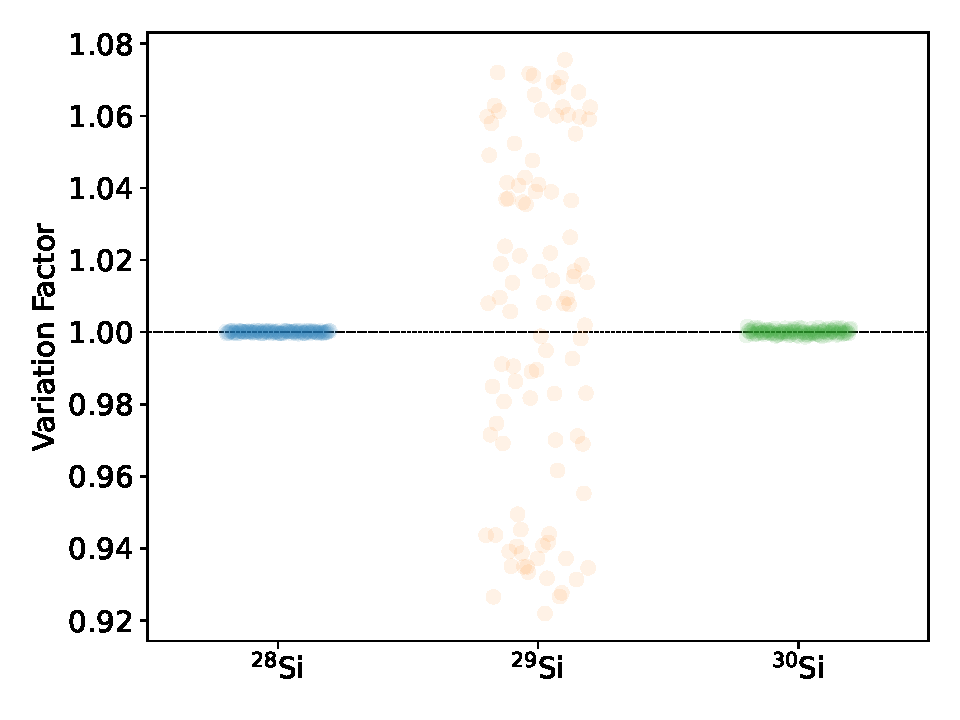
\includegraphics[width=0.7\textwidth]{figs/M20Z1E-2_mcyieldresult.pdf}
    \caption{Monte Carlo result of stellar nucleosynthesis yields in the stellar model with initial mass $M_{ZAM}/\msun =20$ and initial metallicity $Z=0.01$ with the same symbols used in Figure \ref{fig:m15z02_yield}. This figure shows that nuclear uncertainties have the largest impact on the \iso{29}{Si} yield while \iso{28,\, 30}{Si} yields remain largely unchanged by the nuclear uncertainties in the stellar model with $M_{ZAM}/\msun =20$, $Z=0.01$.}
    \label{fig:m20z01_yield}
\end{figure}



\section{Galactic Chemical Evolution of Silicon Isotopes} \label{gce_result}

I calculate the GCE of silicon isotopes using OMEGA+ with stellar yields modified based on the variation factor shown in Section \ref{yield_result}. As shown in Figure \ref{gce_result}, the nuclear uncertainties do affect the GCE of silicon isotopes. Most of the mainstream grains are formed $\ll 0.5$ billion years prior to the formation of the solar system (\citealt{Heck2020}). By taking into account the lifetime of the parent stars, I focus on the slope $\alpha$ of the silicon-correlation line (i.e., $\del{29}{28}{Si} = \alpha \times \del{30}{28}{Si} + \beta$) for the GCE 1.8-0.5 billion years prior to the formation of the solar system. The slope is calculated using, 
\begin{equation}
    \alpha = \frac{[\del{29}{28}{Si}]_f-[\del{29}{28}{Si}]_i}{[\del{30}{28}{Si}]_f-[\del{30}{28}{Si}]_i},
\end{equation}
where $[\del{29,\, 30}{28}{Si}]_f$ and $[\del{29,\, 30}{28}{Si}]_i$ are the values at the last and first data points respectively.

The maximum slope I obtained is 0.42 from the Monte Carlo simulations. The minimum slope I obtained is 0.40. The slope of the model using the default NuGrid yield set is 0.41. I see that the nuclear uncertainties do affect the slope of the silicon-correlation line and yield  up to $\sim 5\%$ variation in the slope of the silicon-correlation line. However, the slope I determined is incompatible with the measurement by \cite{Zinner2007}, which gives a slope of $1.37 \pm 0.01$. Nonetheless, my result provides a large step forward in explaining the discrepancy between the slope of the silicon-correlation line derived from GCE models and the Si mainstream line. 

It is important to note that the slope predicted using the default NuGrid model is much lower than predicted by using other stellar yield sets. This is due to the effect of the convective oxygen-carbon (O-C) shell mergers that occur in stellar models with $M_{ZAM}/\msun = 12, 15, 20$ at $Z=0.01$ and $M_{ZAM}/\msun = 15$ at $Z=0.02$ (\citealt{Ritter_2018}). Due to the 3D nature of the shell mergers, the 1D stellar evolution code used in the NuGrid models is not able to capture the accurate behaviors of the rapidly evolving convective-reactive flows (\cite{Andrassy_2019}). This will lead to an overestimation of the \iso{30}{Si} production in the models where the O-C shell mergers occur. The overproduction of \iso{30}{Si} will therefore significantly lower the slope of the silicon-correlation line. Nonetheless, my study poses a first estimate on the relative uncertainties on the slope of the silicon-correlation line due to the nuclear uncertainties. 

Moreover, for the $(n, \gamma)$ reactions, I only considered the experimental uncertainties without considering the discrepancy between the measurements of different experiments. For example, the rates for $(n,\gamma)$ on \iso{28}{Si} and \iso{30}{Si} by \cite{guber2003} is much lower than determined by \cite{BAO200070}. In my work, I used only the $(n, \gamma)$ rates determined by \cite{guber2003} and their experimental uncertainties. An increase in the $(n, \gamma)$ rate on \iso{28}{Si} and on \iso{30}{Si} can potentially lead to an increase in the production of \iso{29}{Si} and the destruction of \iso{30}{Si}, which further increases the slope of the silicon-correlation line. 

\begin{figure}[H]
    \begin{subfigure}[c]{0.49\textwidth}
        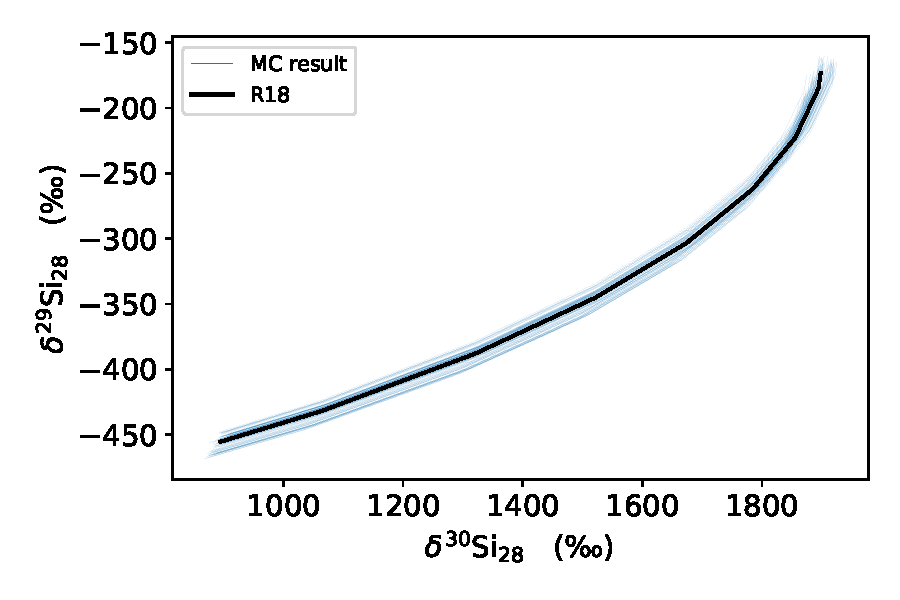
\includegraphics[width=\textwidth]{figs/GCE_1.pdf}
    \end{subfigure}
    \begin{subfigure}[c]{0.49\textwidth}
        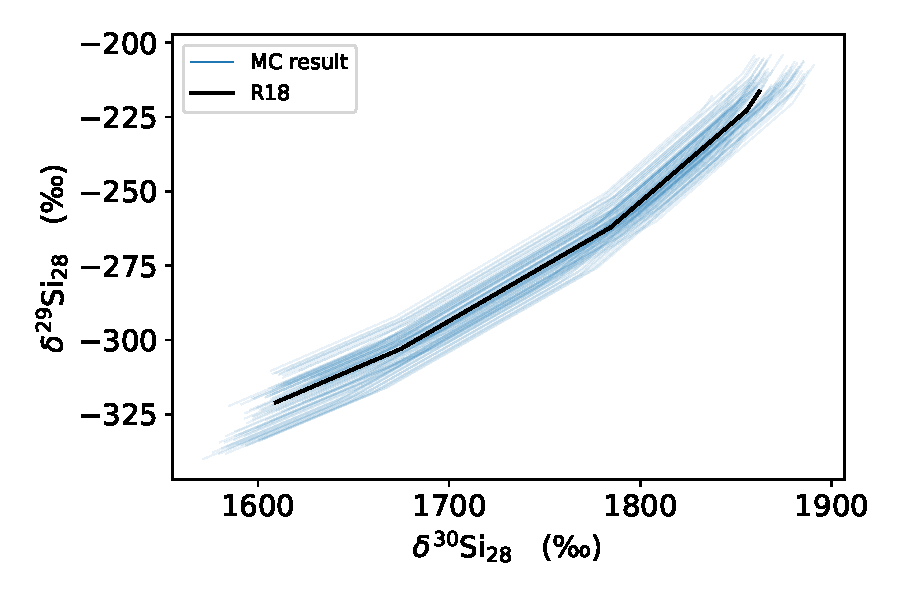
\includegraphics[width=\textwidth]{figs/GCE_2.pdf}
    \end{subfigure}
    \centering
    \begin{subfigure}[c]{0.49\textwidth}
        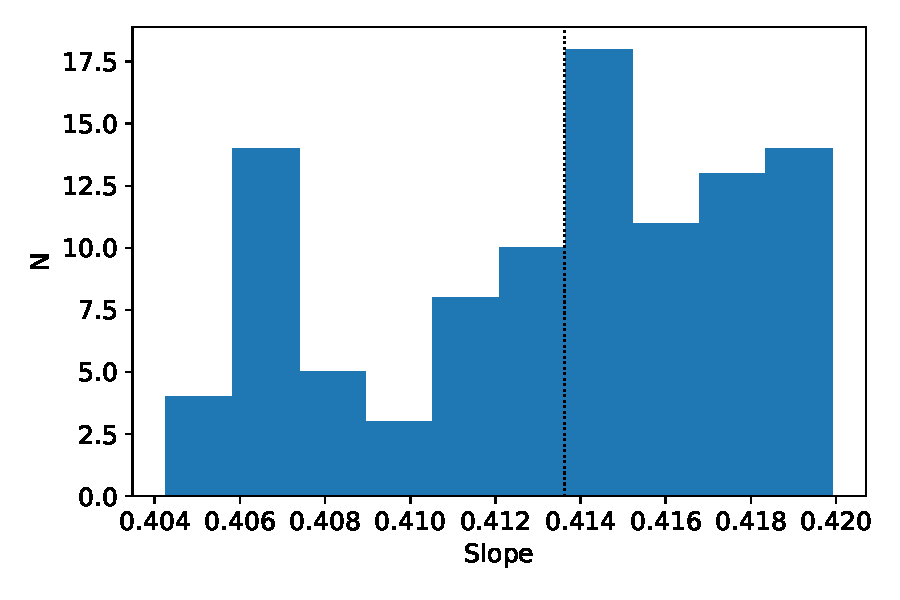
\includegraphics[width=\textwidth]{figs/slope.pdf}
    \end{subfigure}
    \begin{subfigure}[c]{0.49\textwidth}
        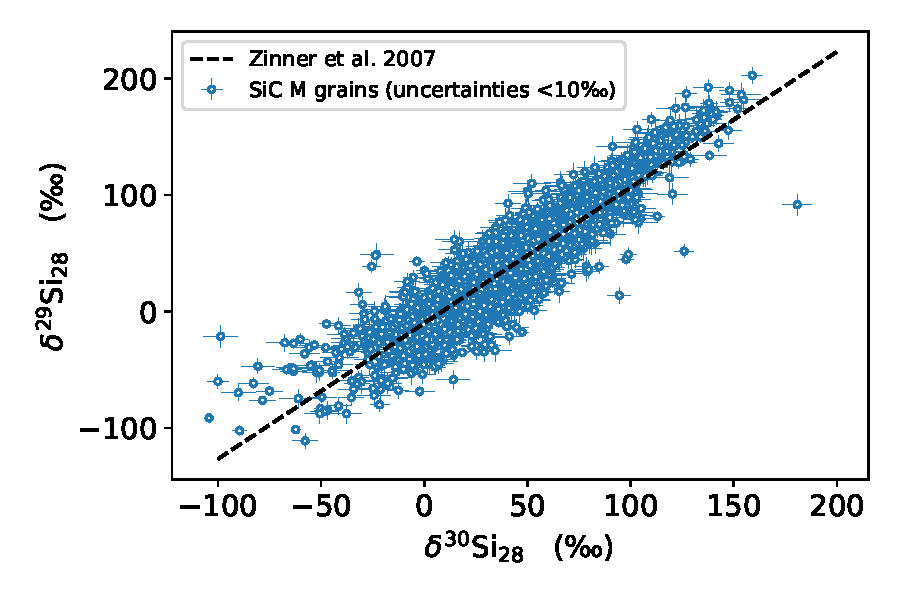
\includegraphics[width=\textwidth]{figs/stardust.pdf}
    \end{subfigure}
    \caption{The Monte Carlo result of the GCE of silicon isotopes. The top left panel shows the GCE of silicon isotopes for the 3 billion years prior to the formation of the solar system. The top right panel shows the GCE of silicon isotopes for the last 500 million years prior to the formation of the solar system. The solid black lines represent the model using the default NuGrid yield set from \citealt{Ritter_2018}. The blue lines represent all Monte Carlo results. The bottom left panel shows the distribution of the slope $\alpha$ of the silicon-correlation line (i.e., $\del{29}{28}{Si} = \alpha \times \del{30}{28}{Si} + \beta$) derived from the Monte Carlo result of the GCE of silicon isotopes 1.8-0.5 billion years prior to the formation of the solar system. The dotted black line represents the slope ($\alpha = 1.25$) derived from the GCE model using the default NuGrid yield set. The bottom right panel shows the SiC mainstream grain data along with the mainstream line (dashed black line) $\del{29}{28}{Si} = 1.37 \times \del{30}{28}{Si} -20\permil$ from \cite{Zinner2007}. This figure shows that nuclear uncertainties do affect the GCE of silicon isotopes. In particular, nuclear uncertainties lead to a $\sim$5\% variation on the slope of the Si-correlation line predicted by the GCE model.}
    \label{fig:gce_result}
\end{figure}



\chapter{Conclusion} \label{conclusion}
My work is the first study to quantify the effects of nuclear uncertainties on the GCE of isotopes. First, my study find that massive stars with initial mass $M/\msun \geq 12$ are responsible for the majority of the silicon produced in the galaxy. In particular, stars with initial mass $15\leq M/\msun \leq 20$ have the highest contribution to \iso{29, \, 30}{Si}. I then find that \iso{29,\, 30}{Si} are produced during explosive oxygen burning in massive stars by comparing the pre-supernova abundances with the post-supernova abundances. I also identify six nuclear reactions that are relevant for silicon production and destruction in the identified regions. 

Using a MC framework, I examine the effects of the nuclear uncertainties on the nucleosynthesis in stellar models with initial mass $M/\msun = 15, 20$ with initial metallicity $Z=0.02, 0.01$. In all the identified silicon-production regions, I show in Section \ref{nucleo_result} that the \iso{29, \, 30}{Si} abundances are affected by the nuclear uncertainties while the \iso{28}{Si} abundances remain largely unchanged. 

Using these nucleosynthesis results, I calculate the modified stellar yields. I show in Section \ref{yield_result} that the \iso{29}{Si} yields are affected by the nuclear uncertainties while the \iso{28,\, 30}{Si} yields remains largely unchanged in three of the models (i.e., $M/\msun = 15,\, 20$ at $Z=0.01$ and $M/\msun = 15$ at $Z=0.02$ models). In $M/\msun = 20$ at $Z=0.02$ model, both the \iso{29}{Si} and \iso{30}{Si} yields are affected by the nuclear uncertainties.

I then perform GCE calculations using the modified stellar yields to determine the effects of nuclear uncertainties on the GCE of silicon isotopes. I find that the nuclear uncertainties can lead to $\sim5\%$ variation in the slope of the silicon-correlation line. The upper limit of the slope is 0.42. The lower limit of the slope is 0.40. The slope I determined is more than a factor of three lower when compared with presolar grain measurement \citep{Zinner2007}; these authors calculated a slope of $1.37\pm 0.01$. This result is likely due to the effect of the convective O-C shell mergers, which lead to a systematic overestimate of the \iso{30}{Si} production in CCSNe with $M_{ZAM}/\msun = 12, 15, 20$ at $Z=0.01$ and $M/\msun = 15$ at $Z=0.02$ (\citealt{Ritter_2018}). Nonetheless, my study poses a bound on the relative uncertainties on the slope of the silicon-correlation line due to the nuclear uncertainties. 

Additionally, my study also works as a proof of concept, showing that it is possible and feasible to combine stellar nucleosynthesis and GCE calculations and perform rate variations in an extended reaction network to quantify the effects of nuclear uncertainties on the GCE of isotopes. 

In the future, I plan to estimate the effect of the O-C shell mergers on the production of silicon isotopes. Furthermore, I will extend this investigation to a wider range of progenitor masses and initial metallicities and investigate the effects of using different sets of experimental nuclear reaction rates. 







\singlespacing
\bibliography{ref}

\end{document}
